\section{Implementation of Front-end Design}

\textbf{Homepage of shop management system in \ref{fig:fig 6.2.1}}\\[1cm]

\begin{figure}[ht]
    \centering  
    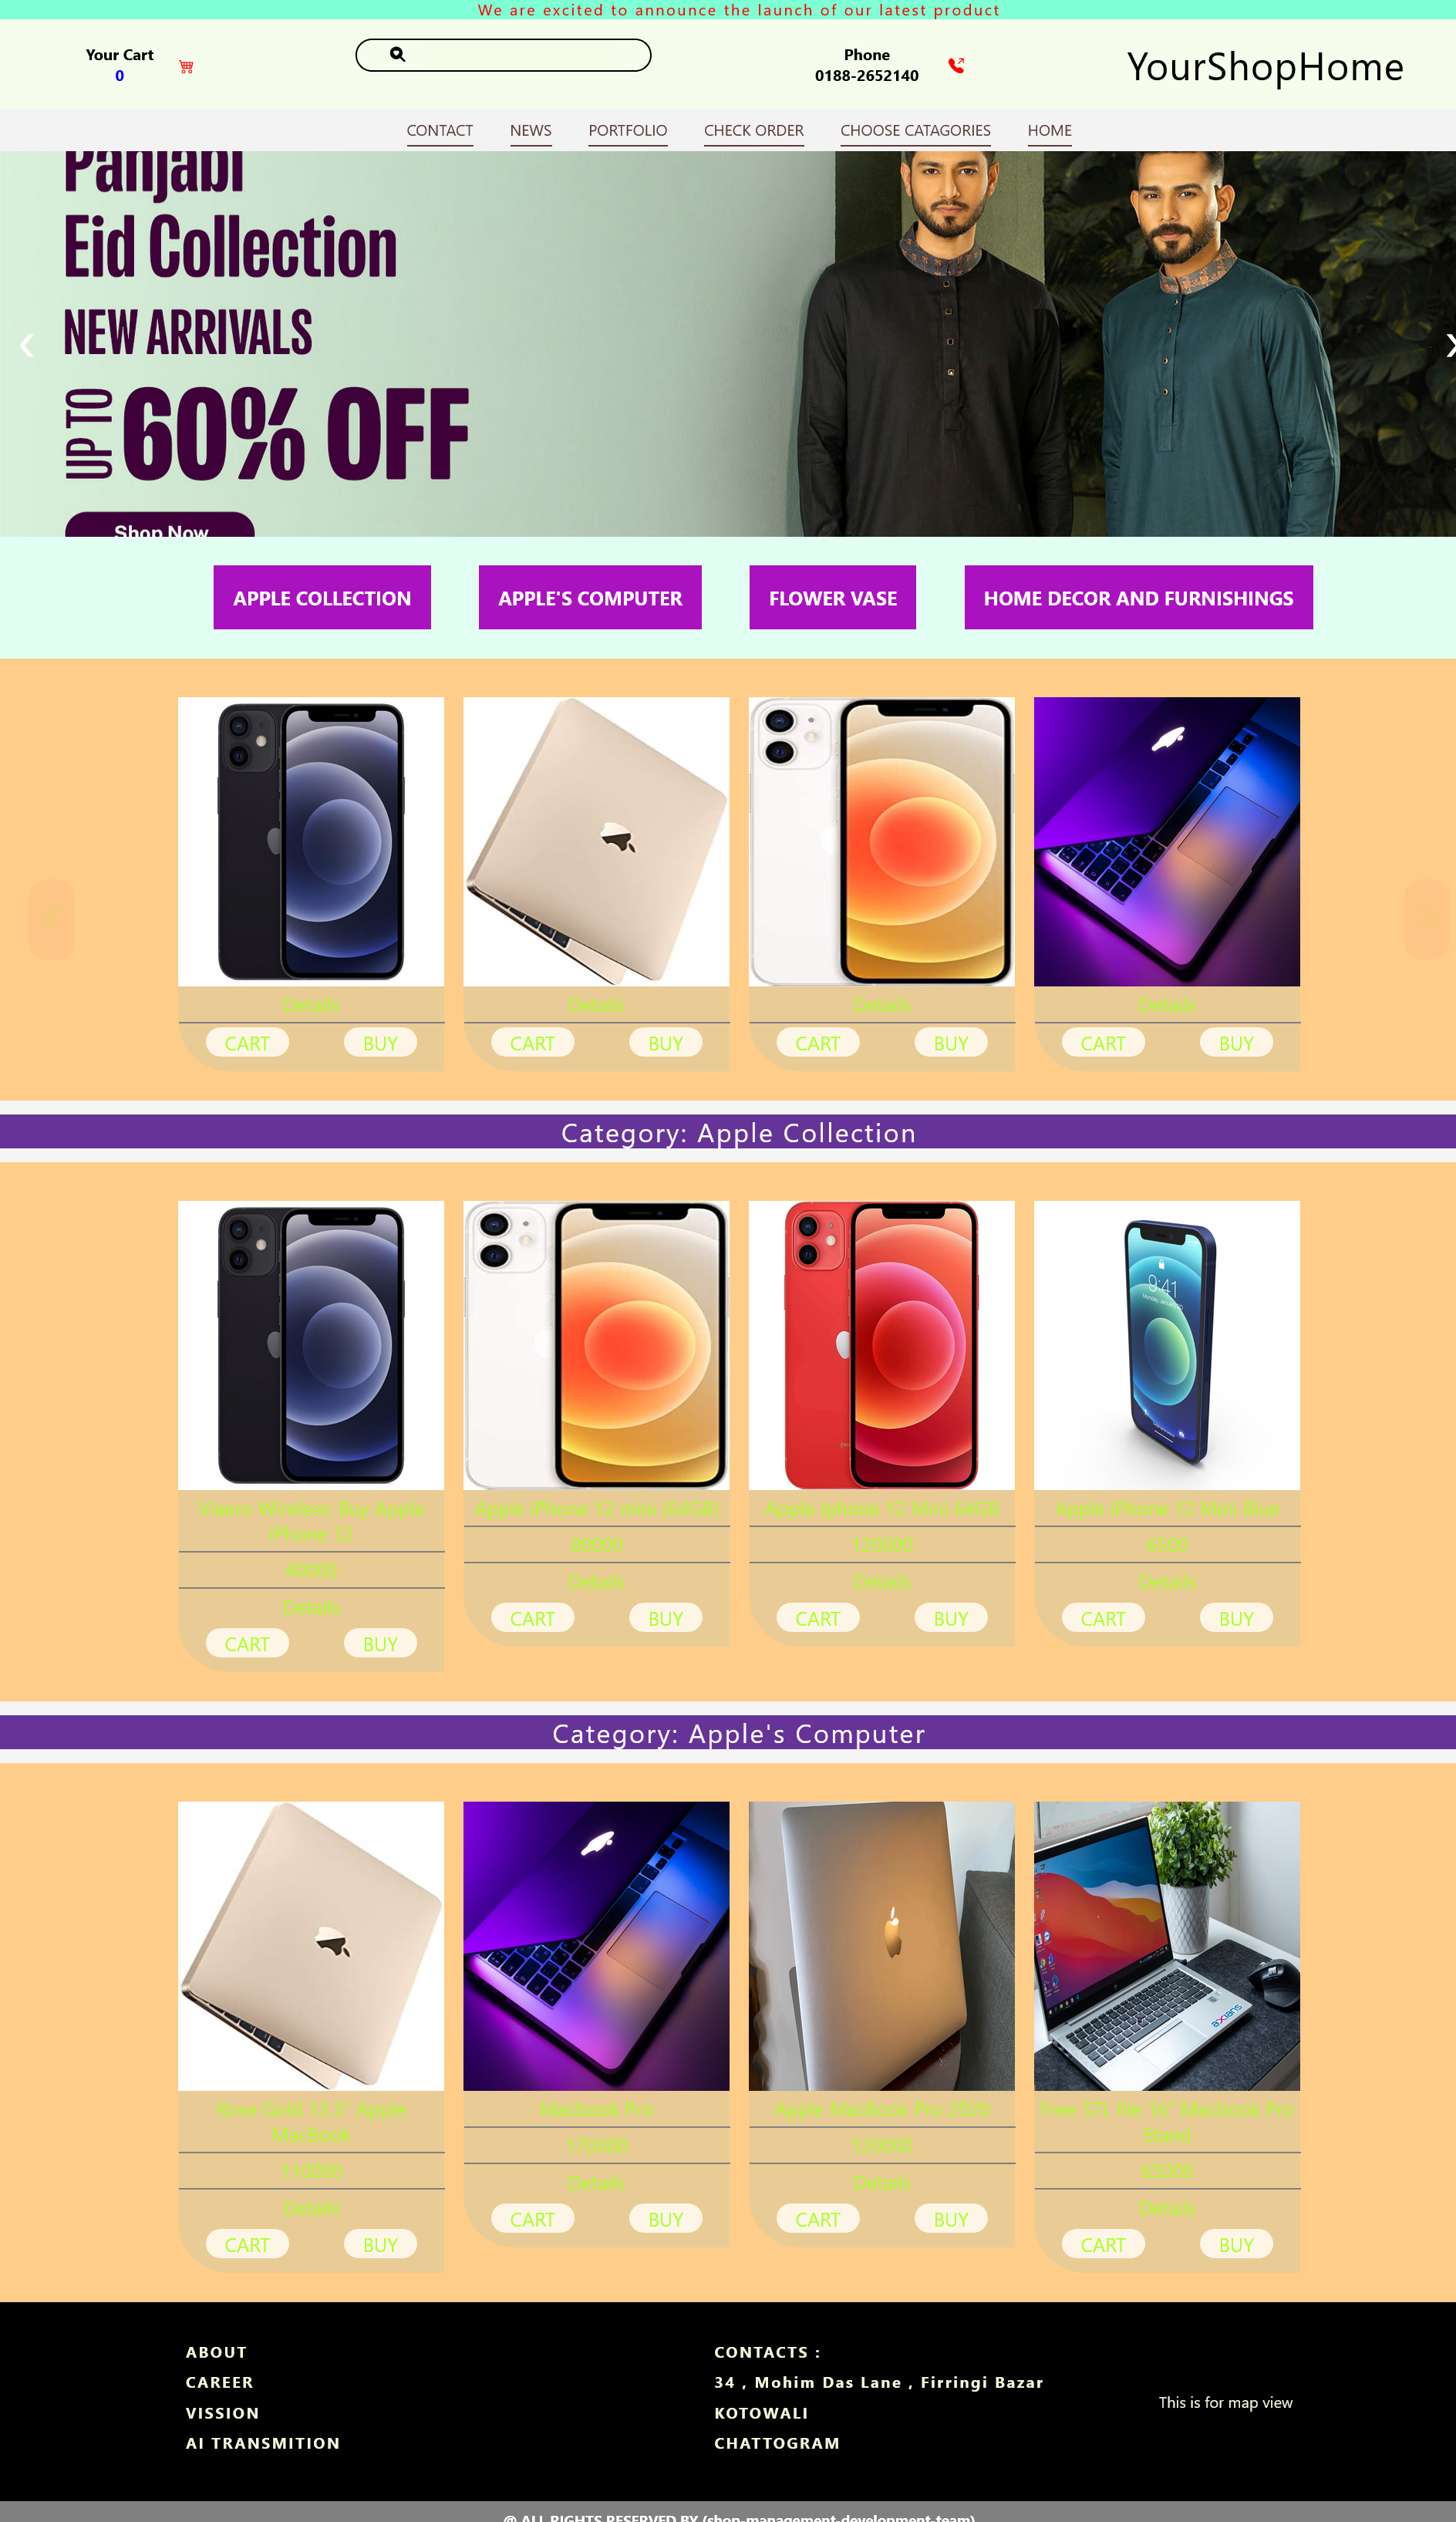
\includegraphics[width=\textwidth, height=0.7\textheight]{designs/Screenshot 2023-06-17 at 14-03-17 Shop management project created by Reshma Dev and Sadia chowdhury.png}    
    \caption{Shop Management Software System Homepage}
    \label{fig:fig 6.2.1}
\end{figure}

\newpage
\vspace{4cm}
\textbf{Design Specification of homepage in \ref{fig:fig6.2.2}}\\[2cm]
\begin{figure}[ht]
    \centering
    \begin{subfigure}[b]{\textwidth}
        \centering
        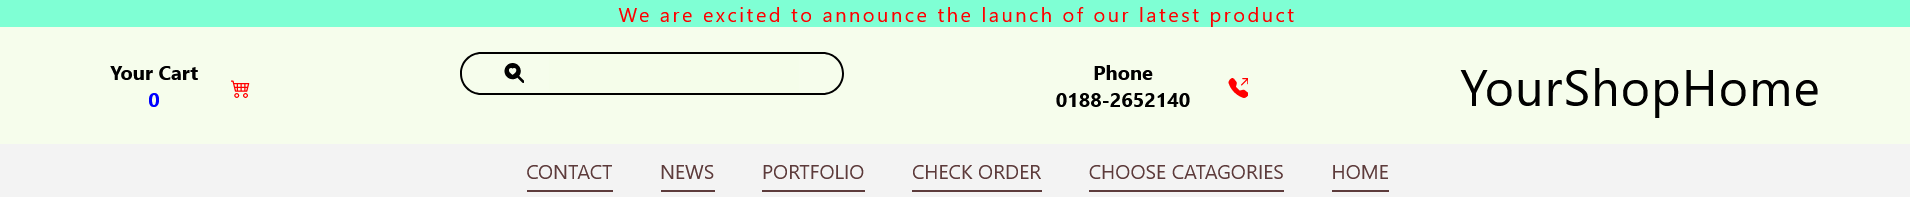
\includegraphics[width=\textwidth]{designs/navigation-pane.png}
        \caption{Navigation Pane}
        \label{fig:6.2.2}
    \end{subfigure}

    \begin{subfigure}[b]{\textwidth}
        \centering
        
\includegraphics[width=\textwidth]{designs/footer.png}
        \caption{Footer}
        \label{fig:6.2.3}
    \end{subfigure}
    \begin{subfigure}[b]{\textwidth}
        \centering        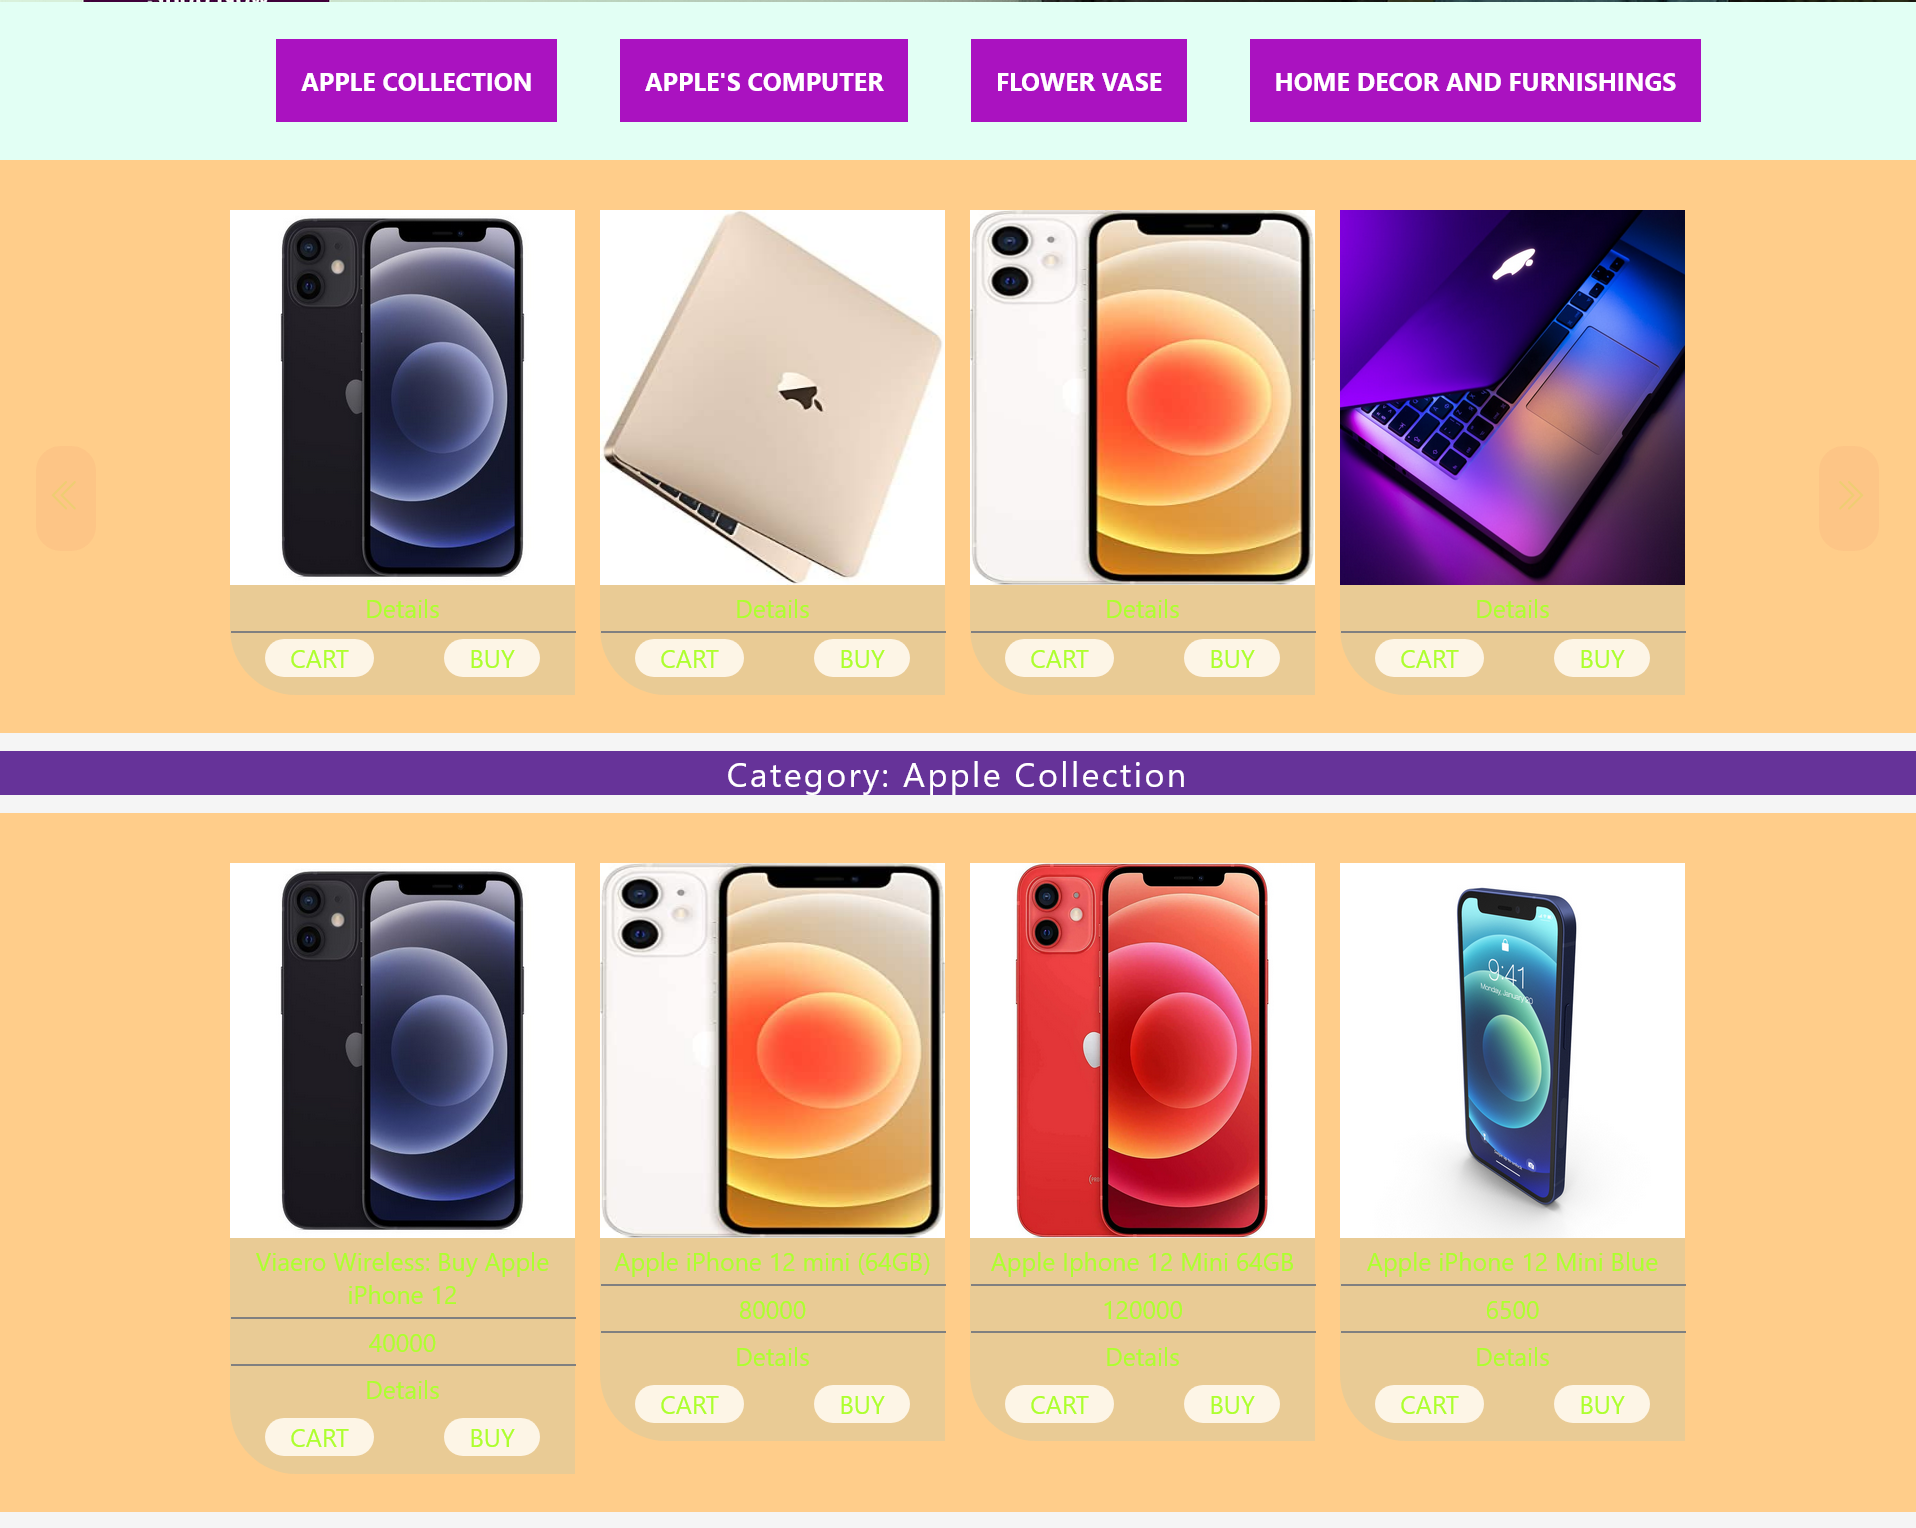
\includegraphics[width=\textwidth,height=0.3\textheight]{designs/catagories.png}
        \caption{Options}
        \label{fig:6.2.4}
    \end{subfigure}

    \begin{subfigure}[b]{\textwidth}
        \centering
        
\includegraphics[width=\textwidth]{designs/carousel.png}
        \caption{Carousel}
        \label{fig:6.2.5}
    \end{subfigure}
    
    
    \caption{Section of Shop management homepage}
    \label{fig:fig6.2.2}
\end{figure}


\newpage
\textbf{Product details section and Product buy form of shop management system in \ref{fig:fig 6.2.6} and \ref{fig:fig 6.2.7}}\\[1cm]
\begin{figure}[ht]
    \centering
    \begin{subfigure}{\textwidth}
          \centering  
           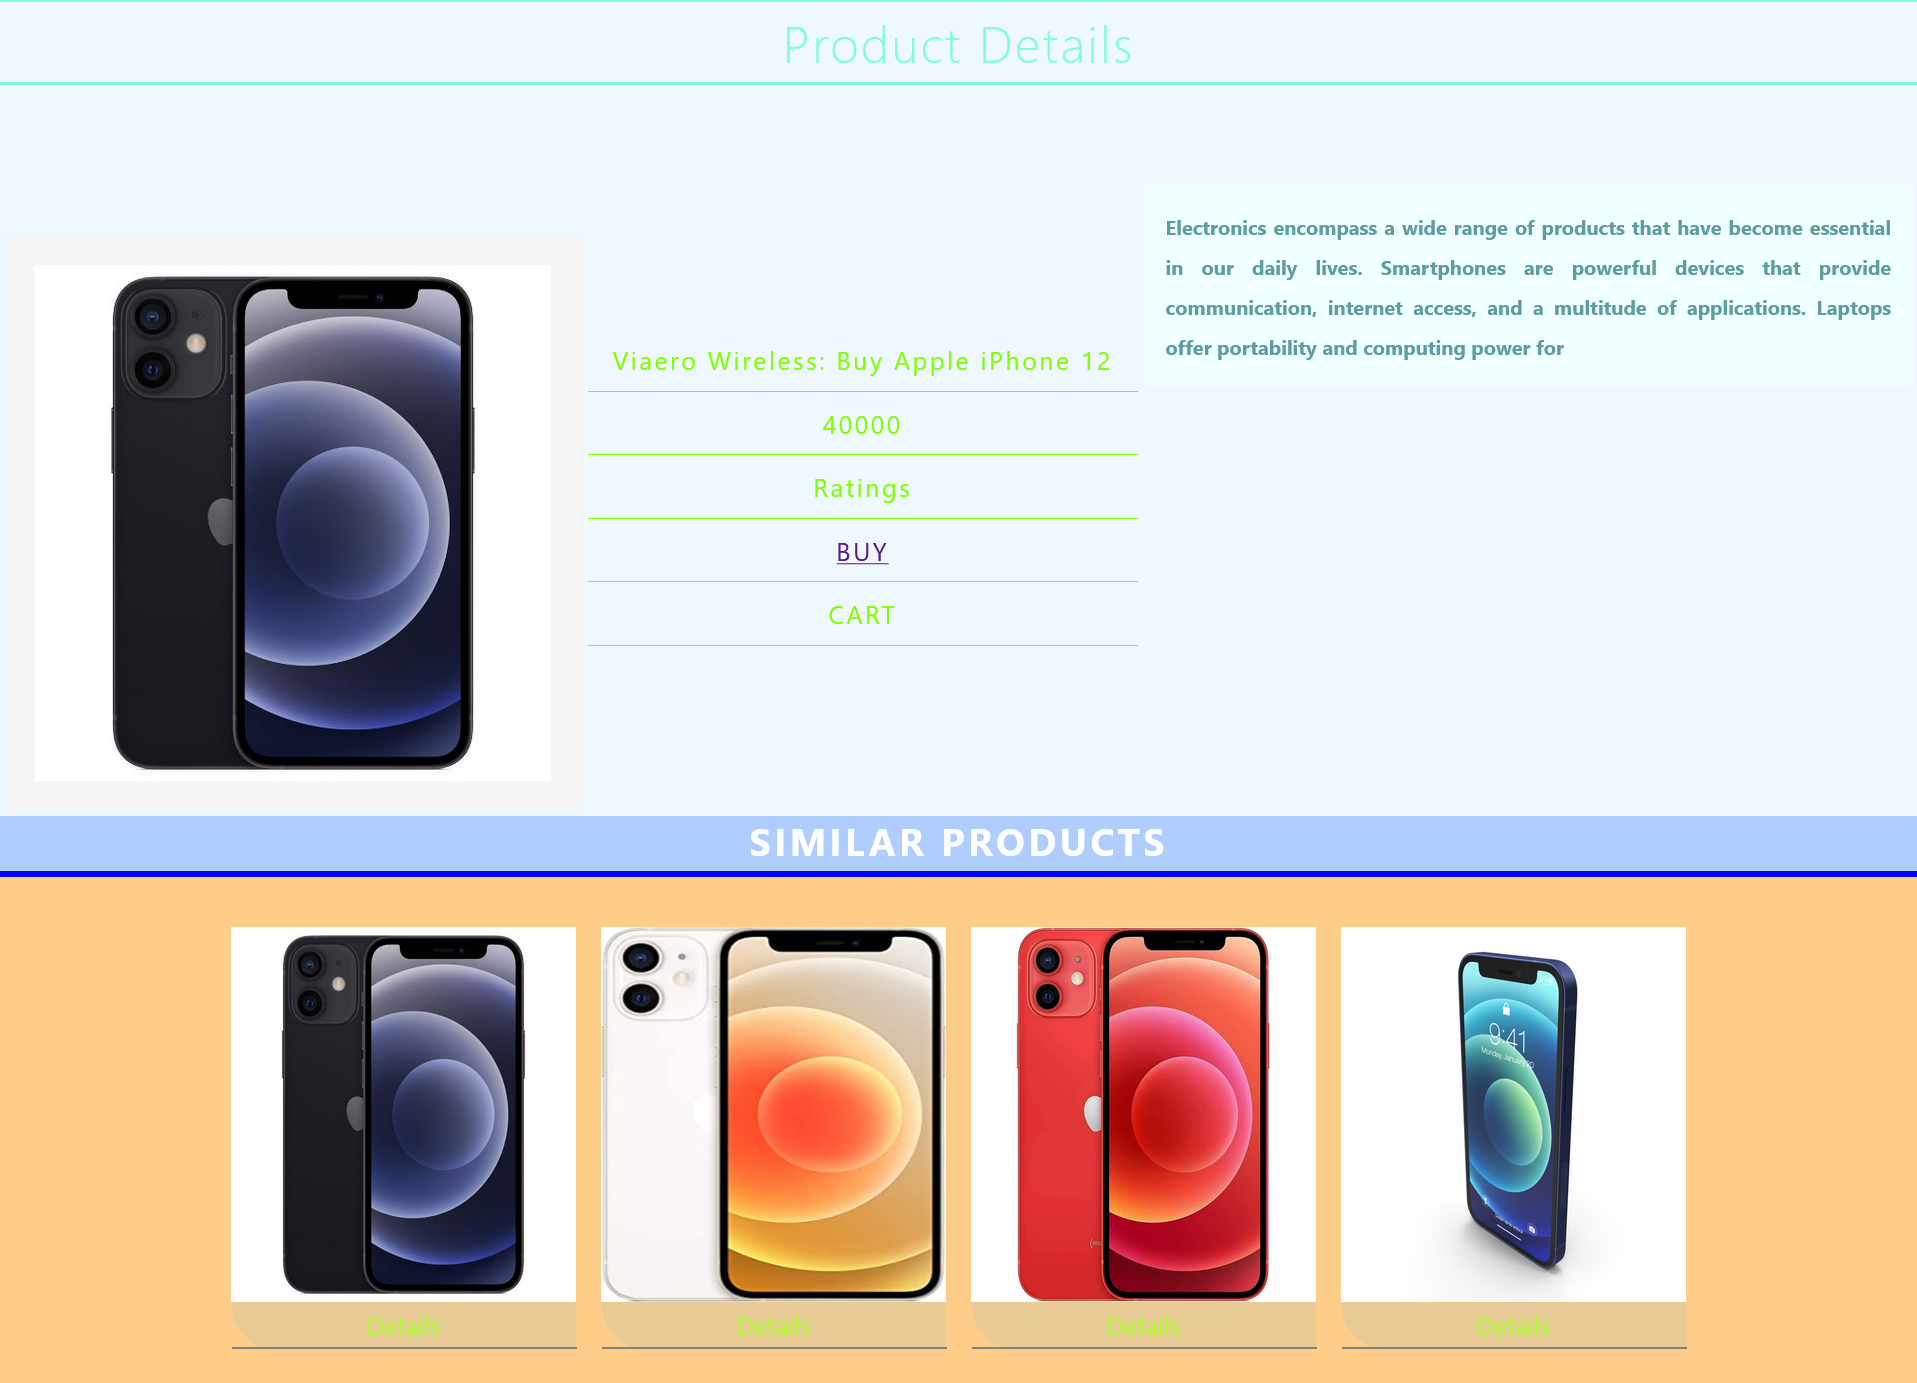
\includegraphics[width=\textwidth]{designs/product details sections.png}   
        \caption{Product Details}
        \label{fig:fig 6.2.6}
    \end{subfigure}

    \begin{subfigure}{\textwidth}
        \centering  
        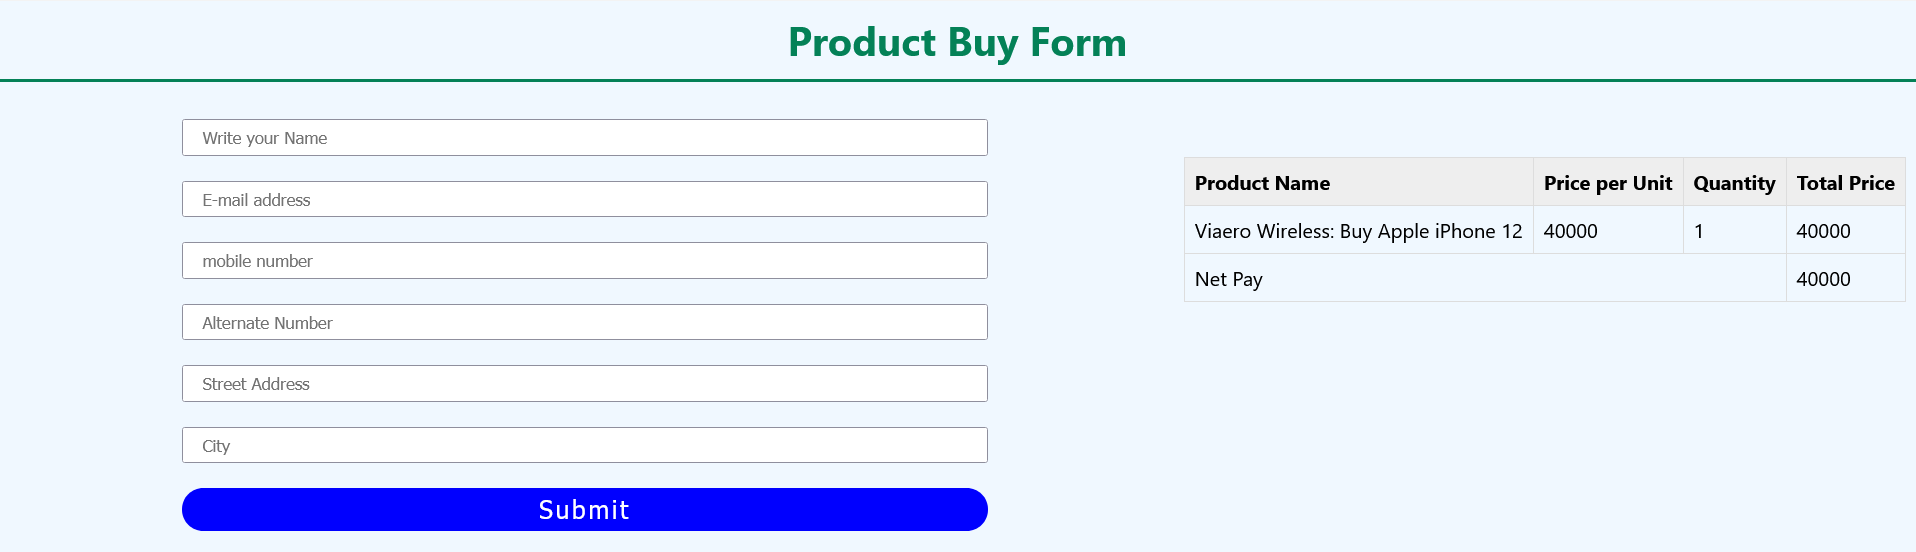
\includegraphics[width=\textwidth ]{designs/product buy form.png}    
        \caption{Product Buy Form}
        \label{fig:fig 6.2.7}
    \end{subfigure}
    
    \caption{Product Details}
    \label{fig:product_details}
\end{figure}

\newpage
\textbf{Submit payment details and create invoice of shop management system in \ref{fig:fig 6.2.8} , \ref{fig:fig 6.2.9}}\\[2cm]
 \begin{figure}[ht]
  \centering  
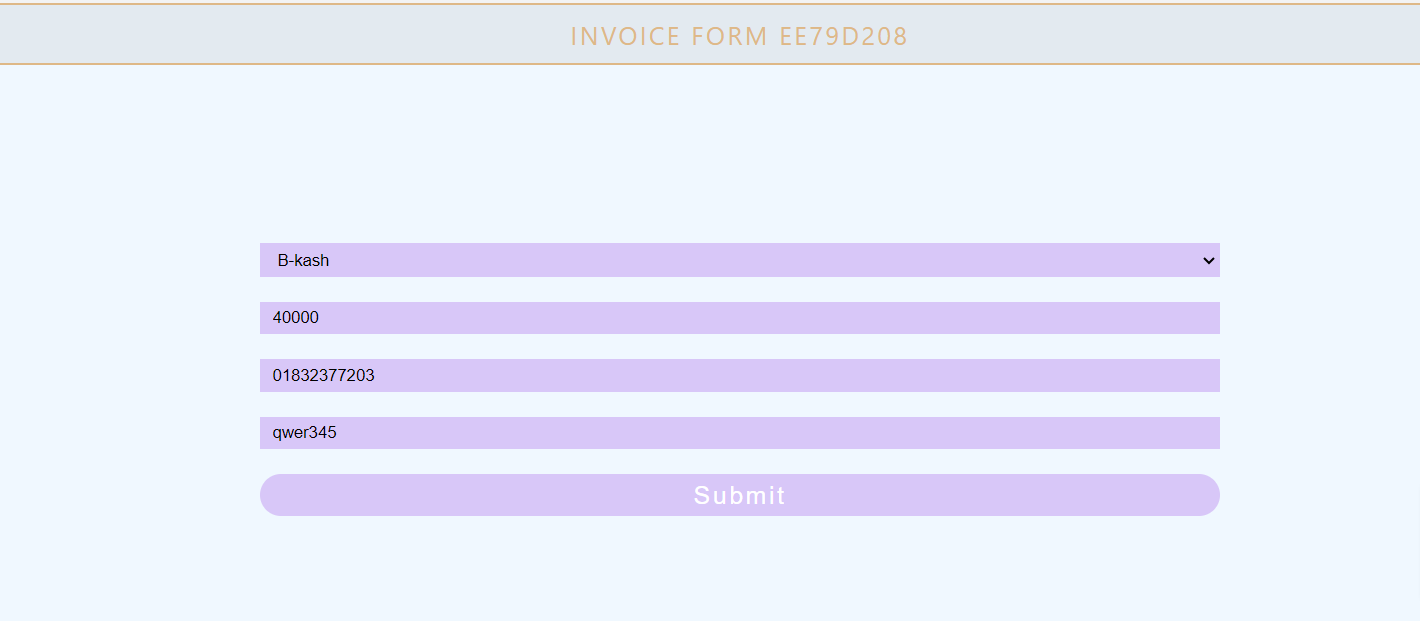
\includegraphics[width=\textwidth,height=0.2\textheight]{designs/submit payment details.png}    
    \caption{Submit Payment Details}
    \label{fig:fig 6.2.8}
 \end{figure}
\begin{figure}[ht]
     \centering  
     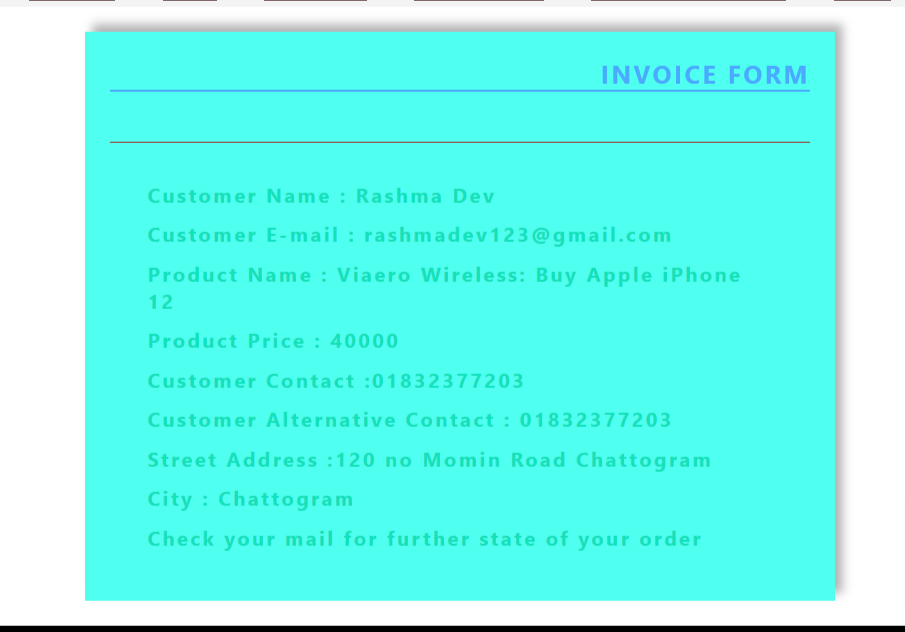
\includegraphics[width=\textwidth]{designs/got invoice.png}    
     \caption{Auto generated invoice}
     \label{fig:fig 6.2.9}
 \end{figure}




\newpage

\textbf{Create order form cart using shop 
management system in \ref{fig:fig 6.2.11}}\\[2cm]
 
\begin{figure}[ht]
    \centering  
    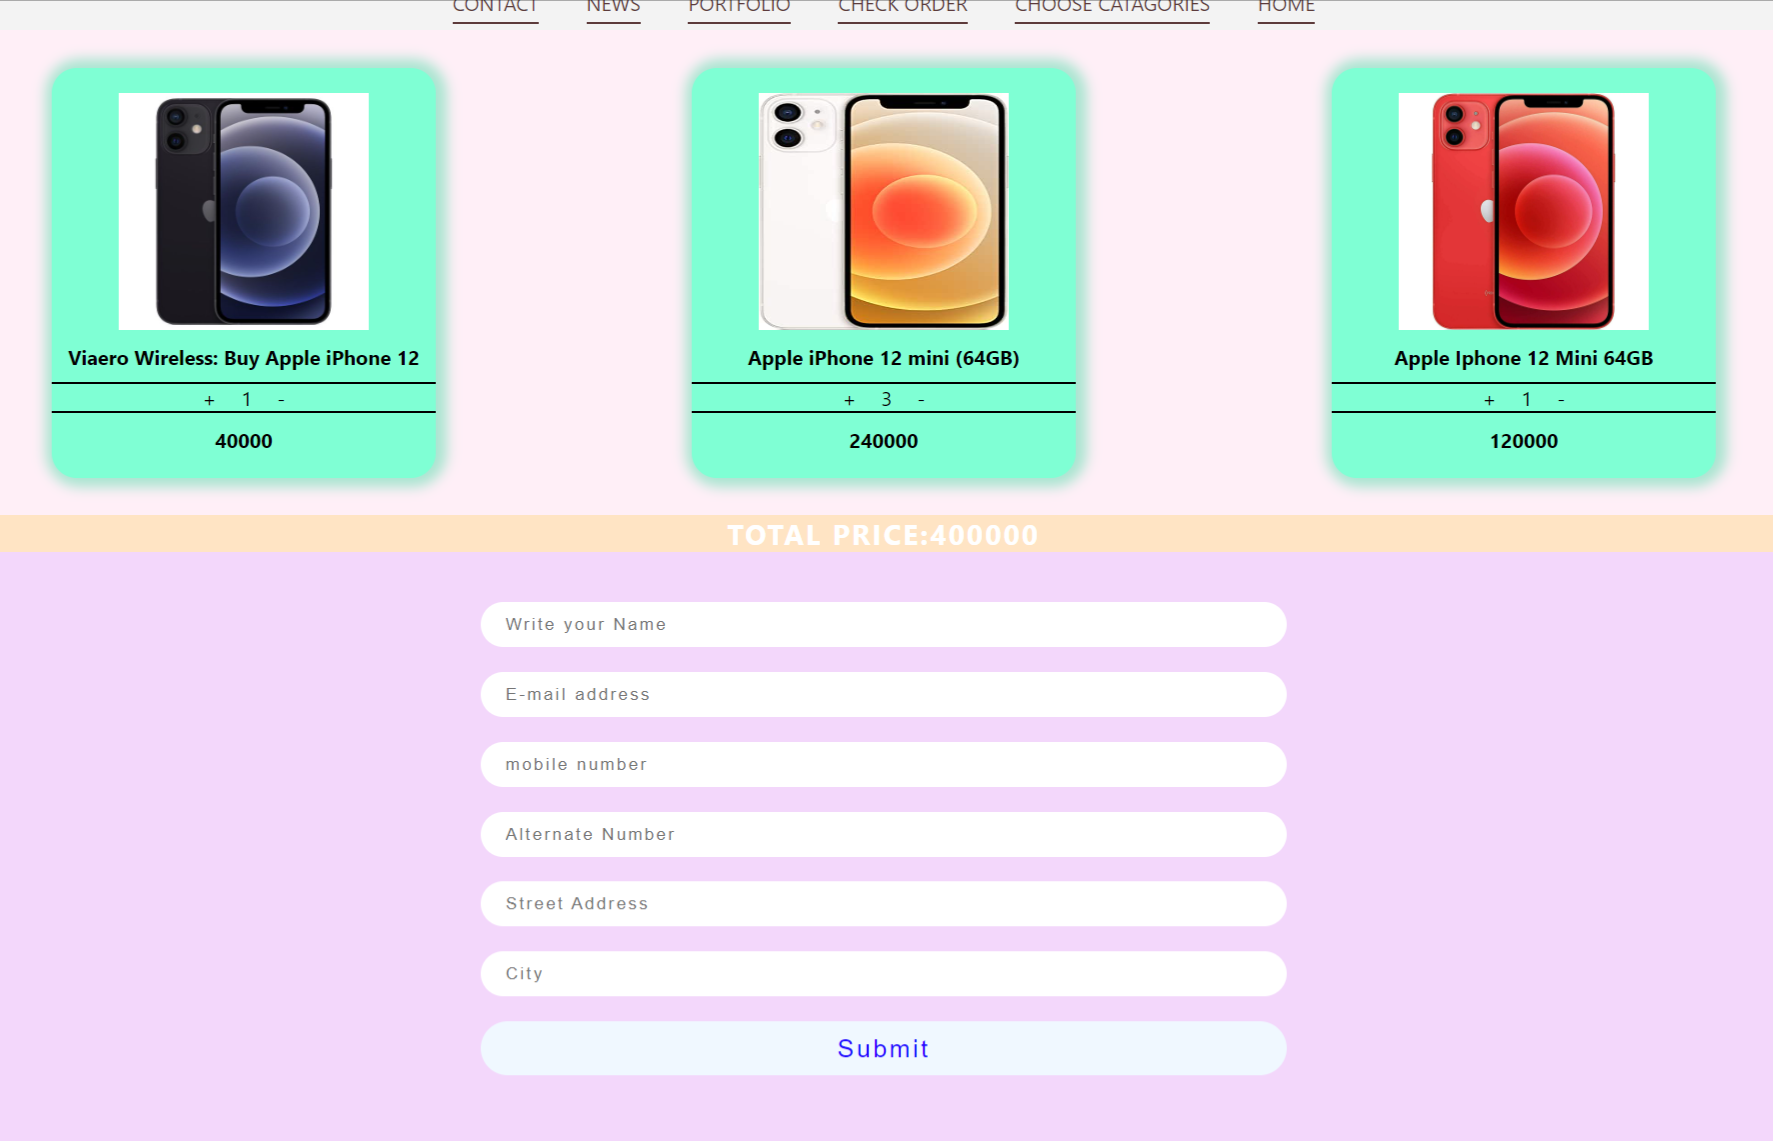
\includegraphics[width=\textwidth]{designs/create_order_from_cart.png}    
    \caption{Cash on delivery method}
    \label{fig:fig 6.2.11}
\end{figure}

\begin{figure}[ht]
    \centering  
    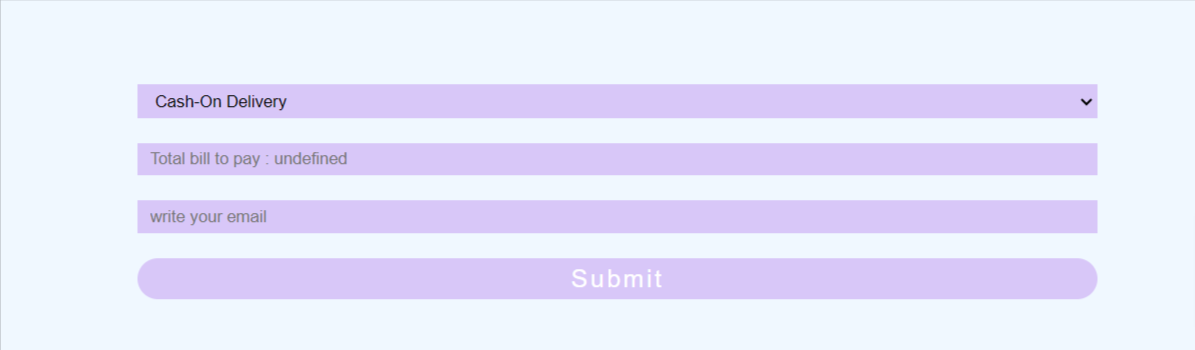
\includegraphics[width=\textwidth]{designs/cash-on-delivery-method.png}    
    \caption{Cash on delivery method}
    \label{fig:fig 6.2.12}
\end{figure}

\newpage
\textbf{Create auto generated invoice form cart using shop management system in \ref{fig:fig 6.2.13}}\\[2cm]
\begin{figure}[ht]
    \centering  
    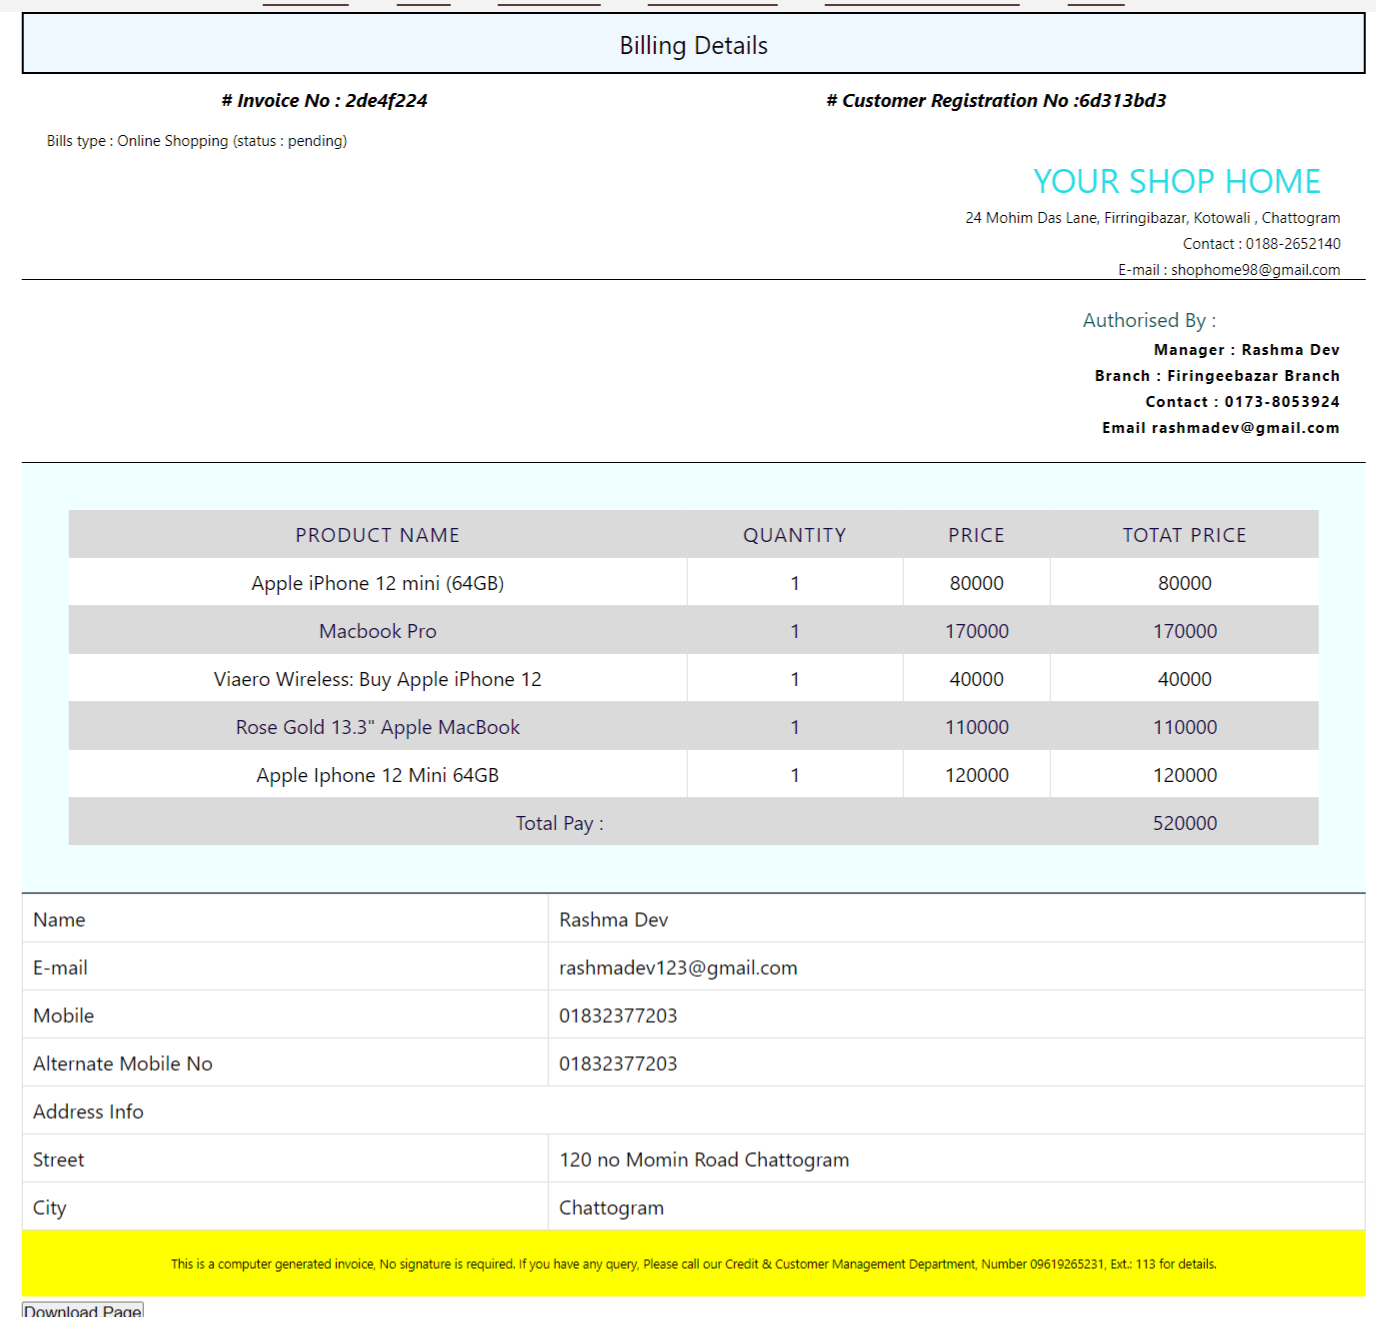
\includegraphics[width=\textwidth, height=0.8\textheight, keepaspectratio]{designs/cart_invoice.png}    
    \caption{Auto generated Cart Invoice}
    \label{fig:fig 6.2.13}
\end{figure}

\newpage
\textbf{Create order form cart using shop management system in \ref{fig:fig6.2.14}}\\
\begin{figure}[ht]
    \centering  
    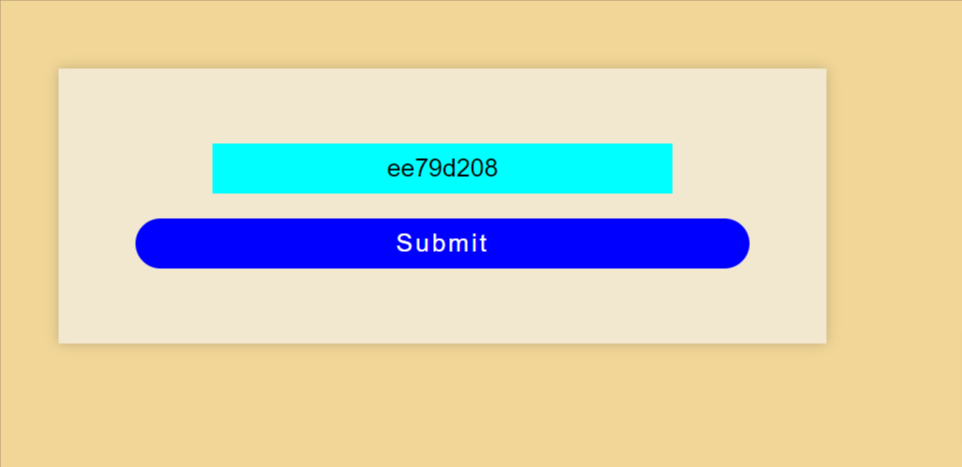
\includegraphics[width=0.6\textwidth, height=0.1\textheight]{designs/inquiry_order_details_by_order_id.png}    
    \caption{Check order state by searching order ID}
    \label{fig:fig6.2.14}
\end{figure}
\\[1cm]
\textbf{Product filtering shop management system in \ref{fig:fig 6.2.15}}\\
\begin{figure}[ht]
    \centering  
    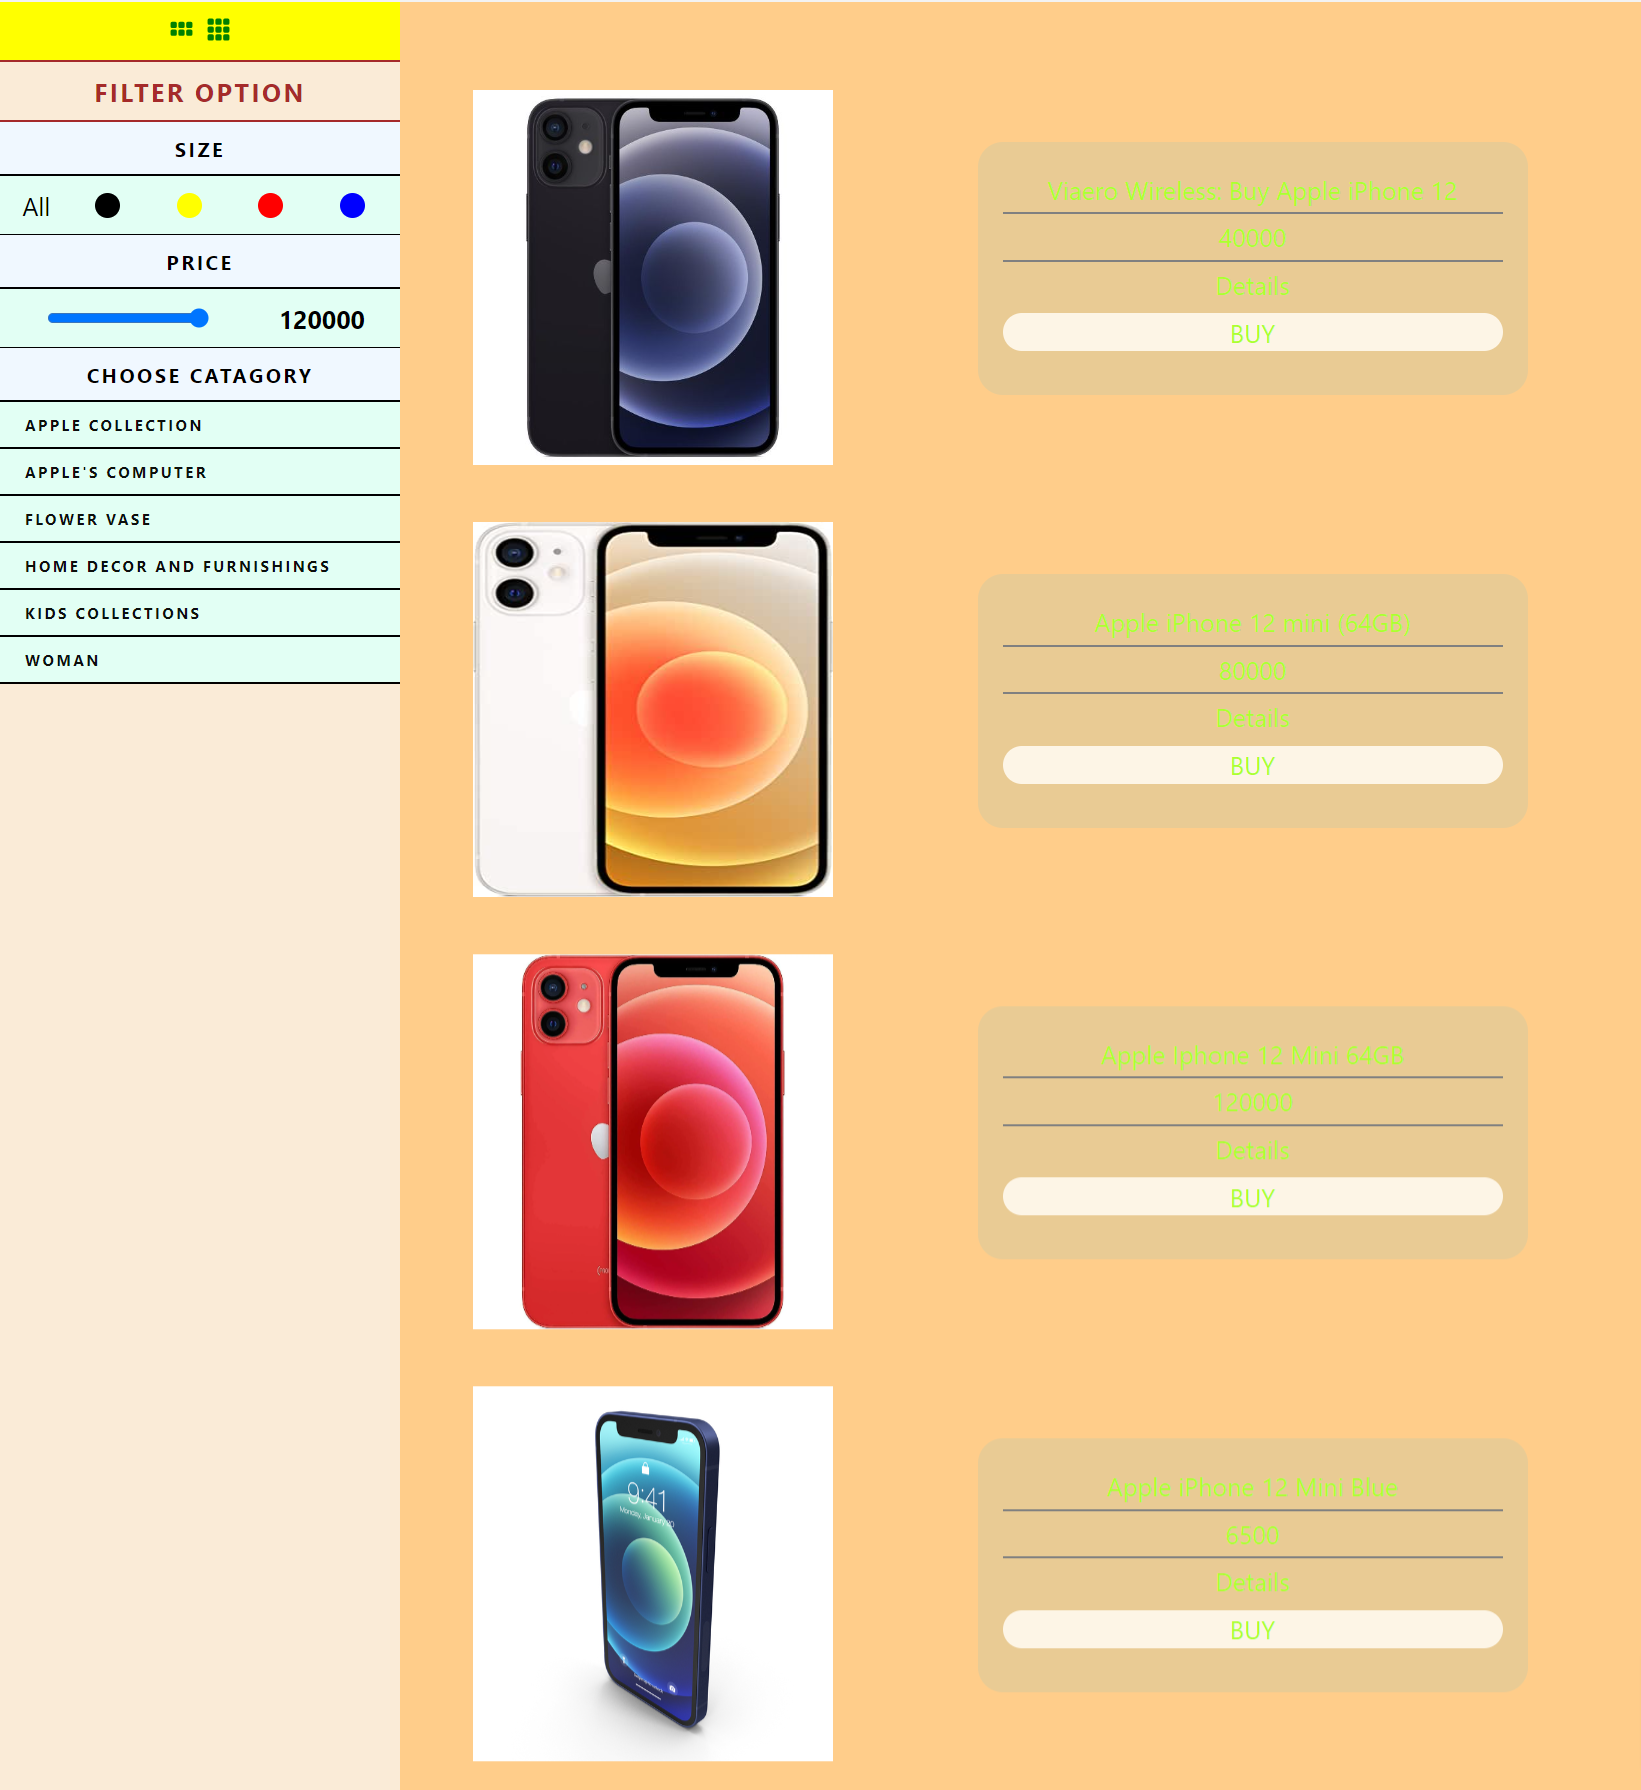
\includegraphics[width=0.9\textwidth,height=0.5\textheight]{designs/product-filtering-options.png}    
    \caption{Product Filtering}
    \label{fig:fig 6.2.15}
\end{figure}

\newpage
\textbf{New Staff Registration in Shop Management System (Figure \ref{fig:fig 6.2.16})}\\
\vspace{2cm}
\begin{figure}[ht]
    \centering  
    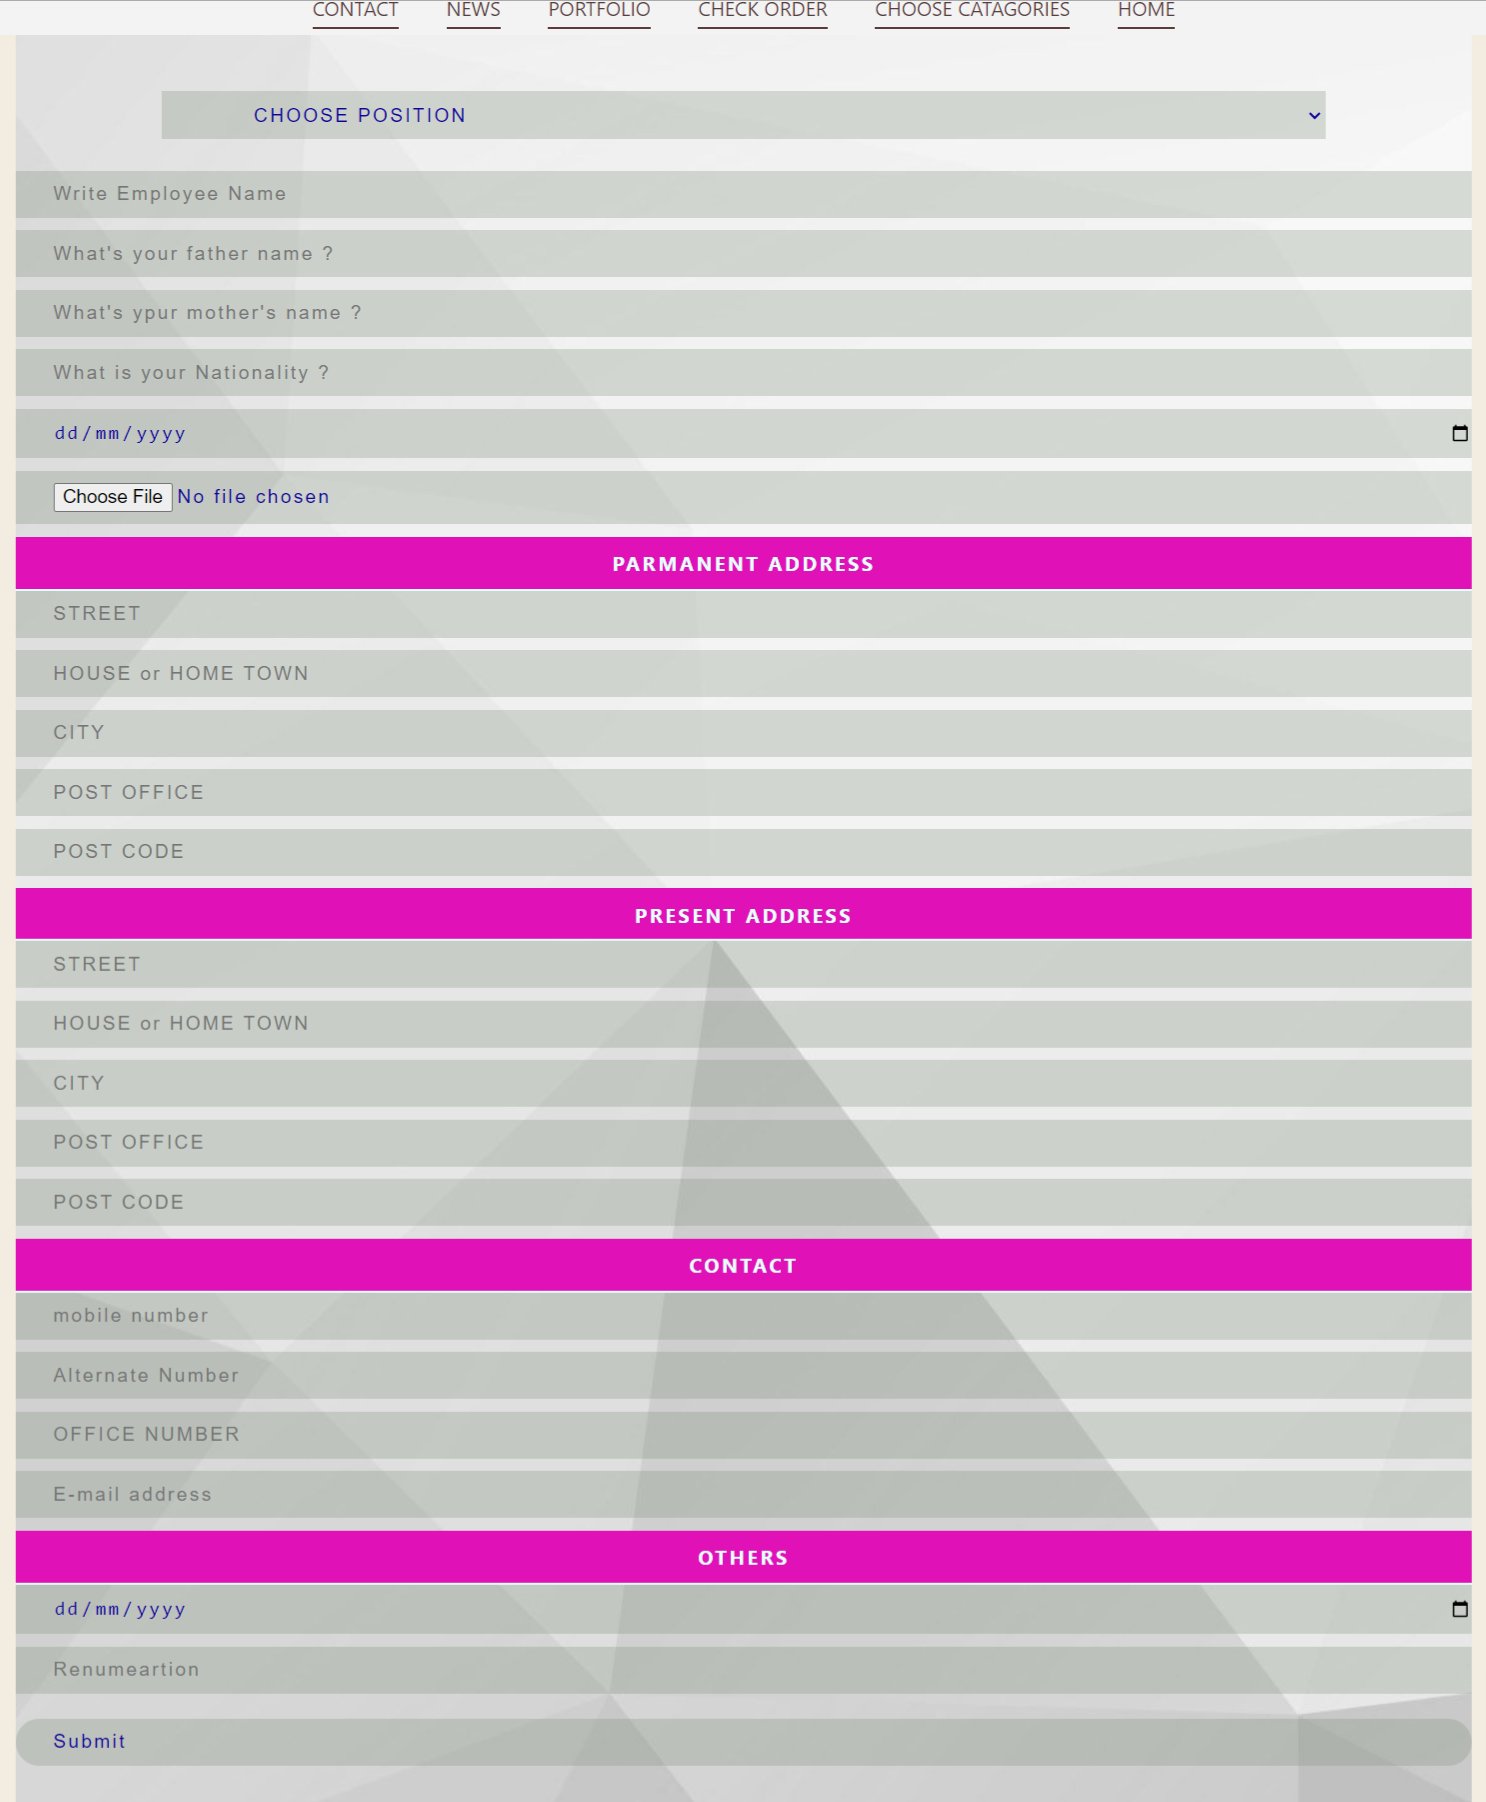
\includegraphics[width=\textwidth, height=0.7\textheight]{designs/staff-registration.png}    
    \caption{Staff Registration Form}
    \label{fig:fig 6.2.16}
\end{figure}

\newpage
\textbf{Staff Login in Shop Management System (Figure \ref{fig:fig 6.2.17})}\\

\begin{figure}[ht]
    \centering  
    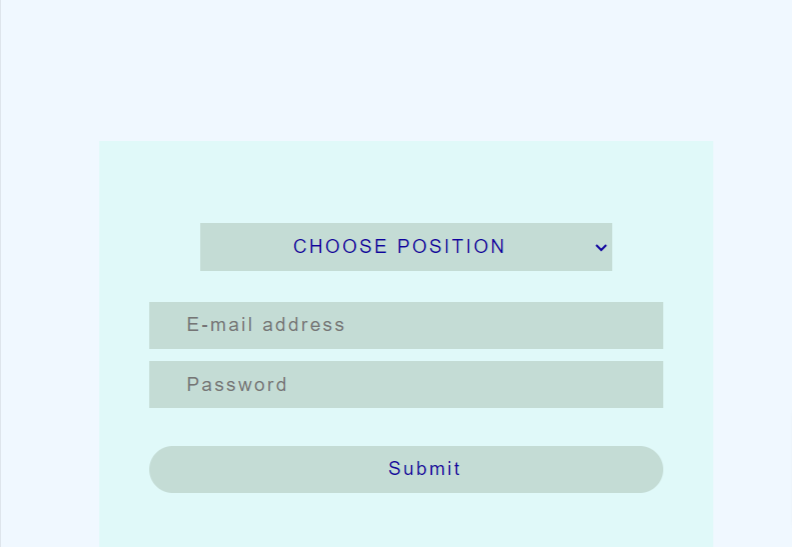
\includegraphics[width=\textwidth, height=0.2\textheight, keepaspectratio]{designs/stafflogin.png}    
    \caption{Staff Login Form}
    \label{fig:fig 6.2.17}
\end{figure}

\begin{figure}[ht]
    \centering  
    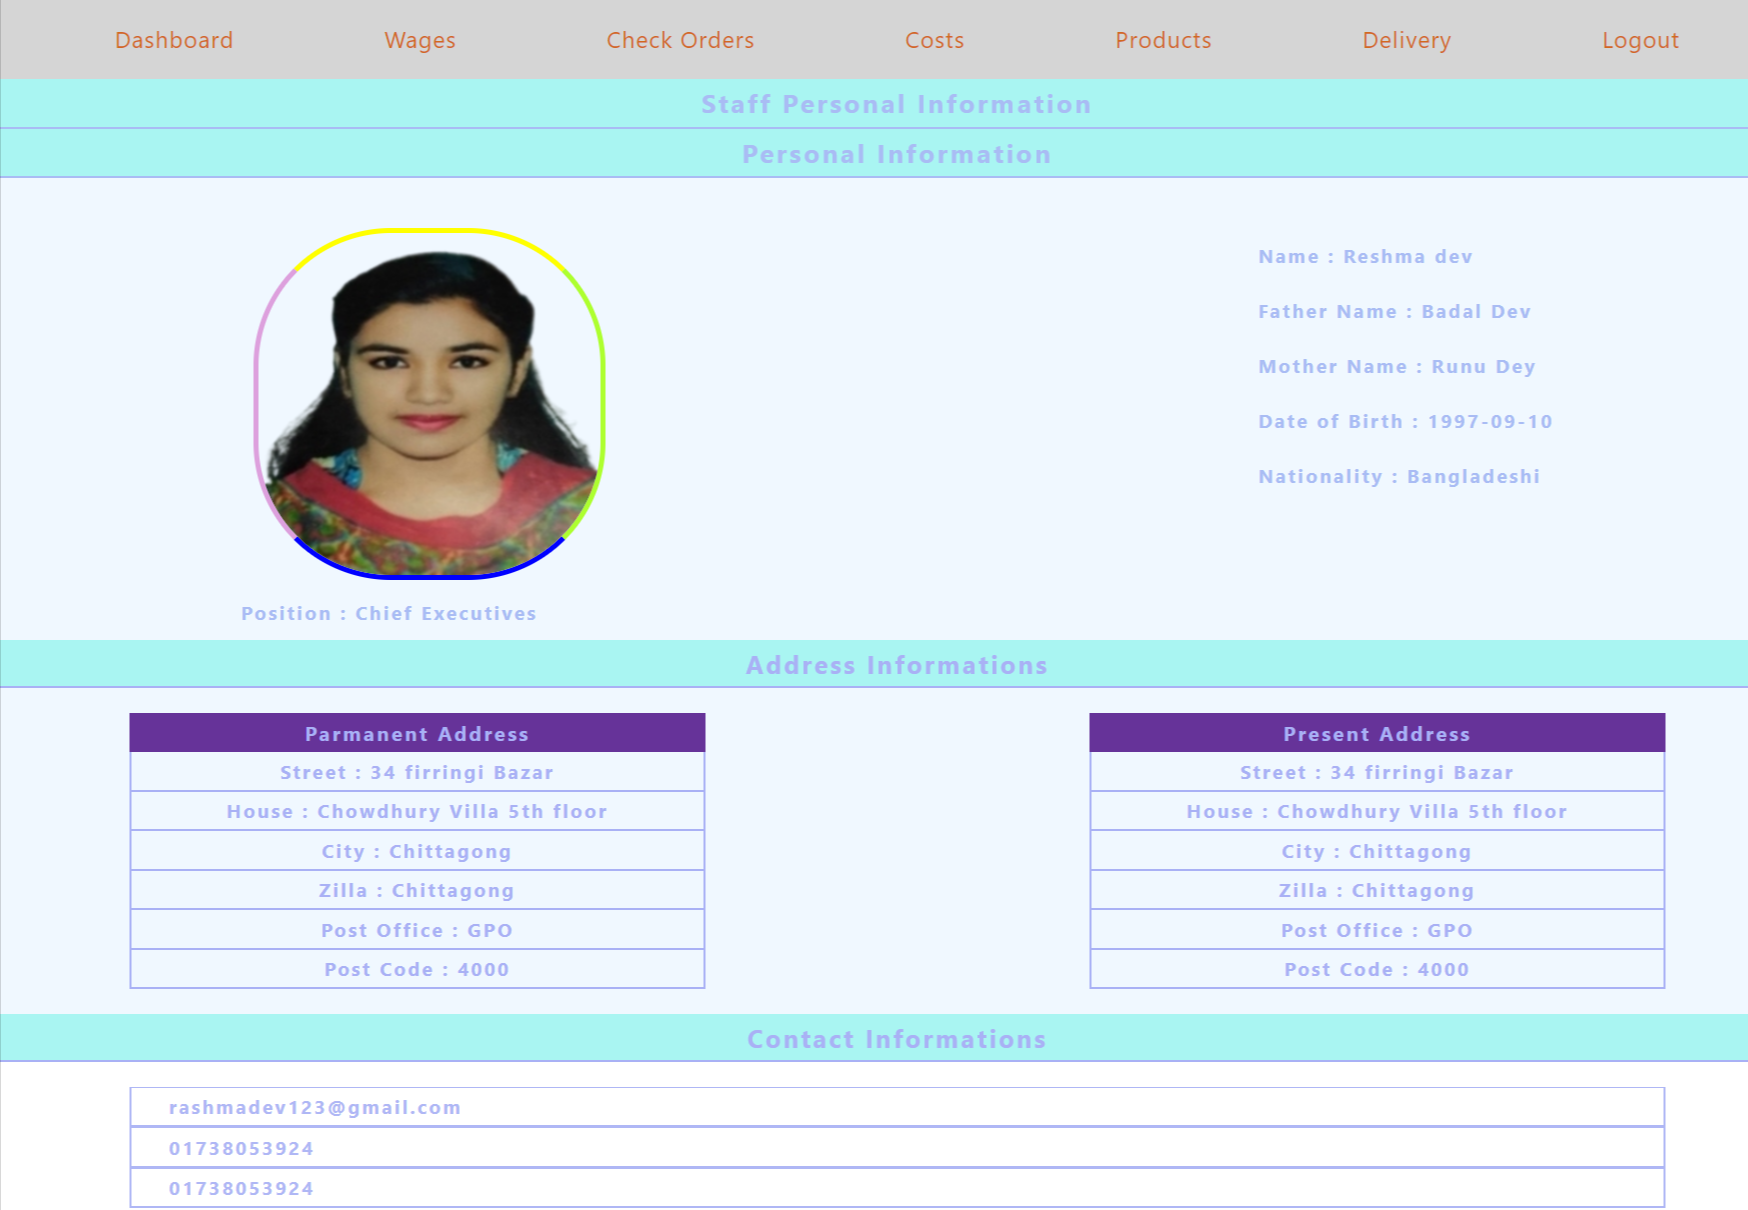
\includegraphics[width=\textwidth, height=0.6\textheight, keepaspectratio]{designs/staff's dashboard.png}    
    \caption{Staff dashboard}
    \label{fig:fig 6.2.18}
\end{figure}

\newpage
\textbf{Revenue implementation visually and manually in Shop Management System (Figure \ref{fig:fig 6.2.19})}\\

\begin{figure}[ht]
    \centering  
    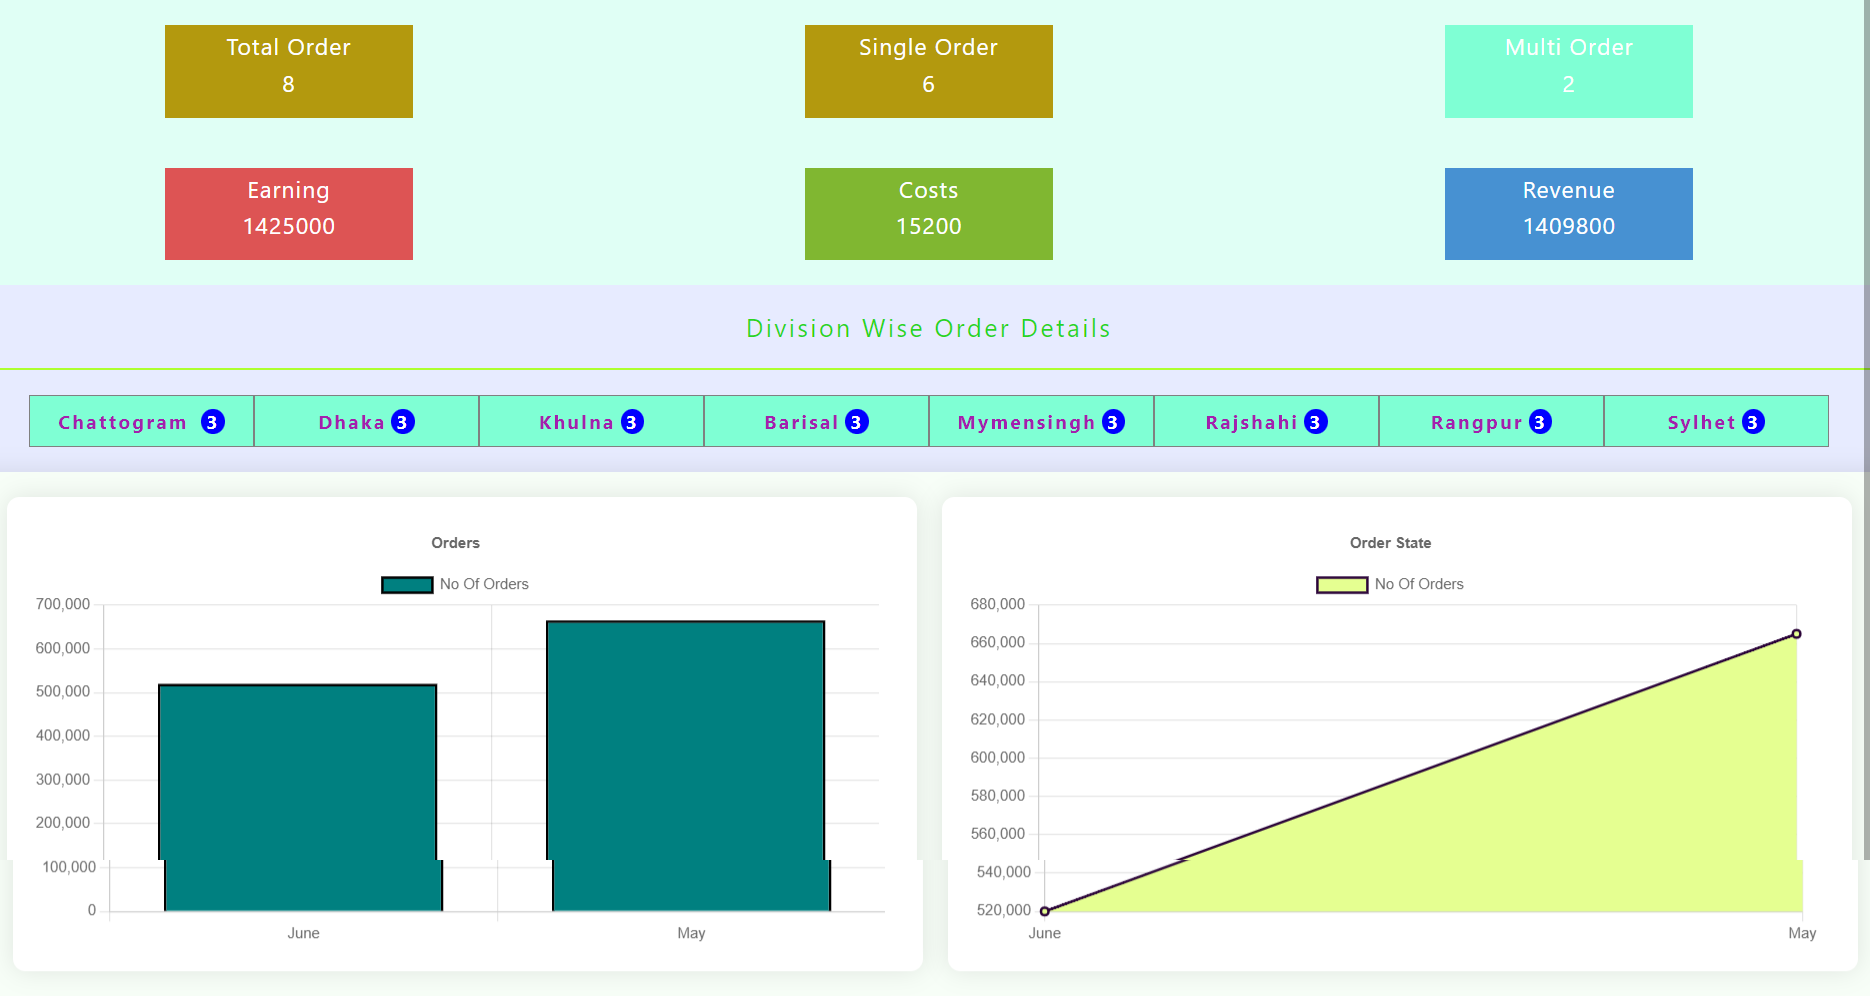
\includegraphics[width=\textwidth, height=0.3\textheight, keepaspectratio]{designs/Reveneue and graph.png}    
    \caption{Visual and Manual Implementations of Revenue}
    \label{fig:fig 6.2.19}
\end{figure}

\vspace{2cm}
\textbf{Validate transaction and orders in Shop Management System (Figure \ref{fig:fig 6.2.20})}\\

\begin{figure}[ht]
    \centering  
    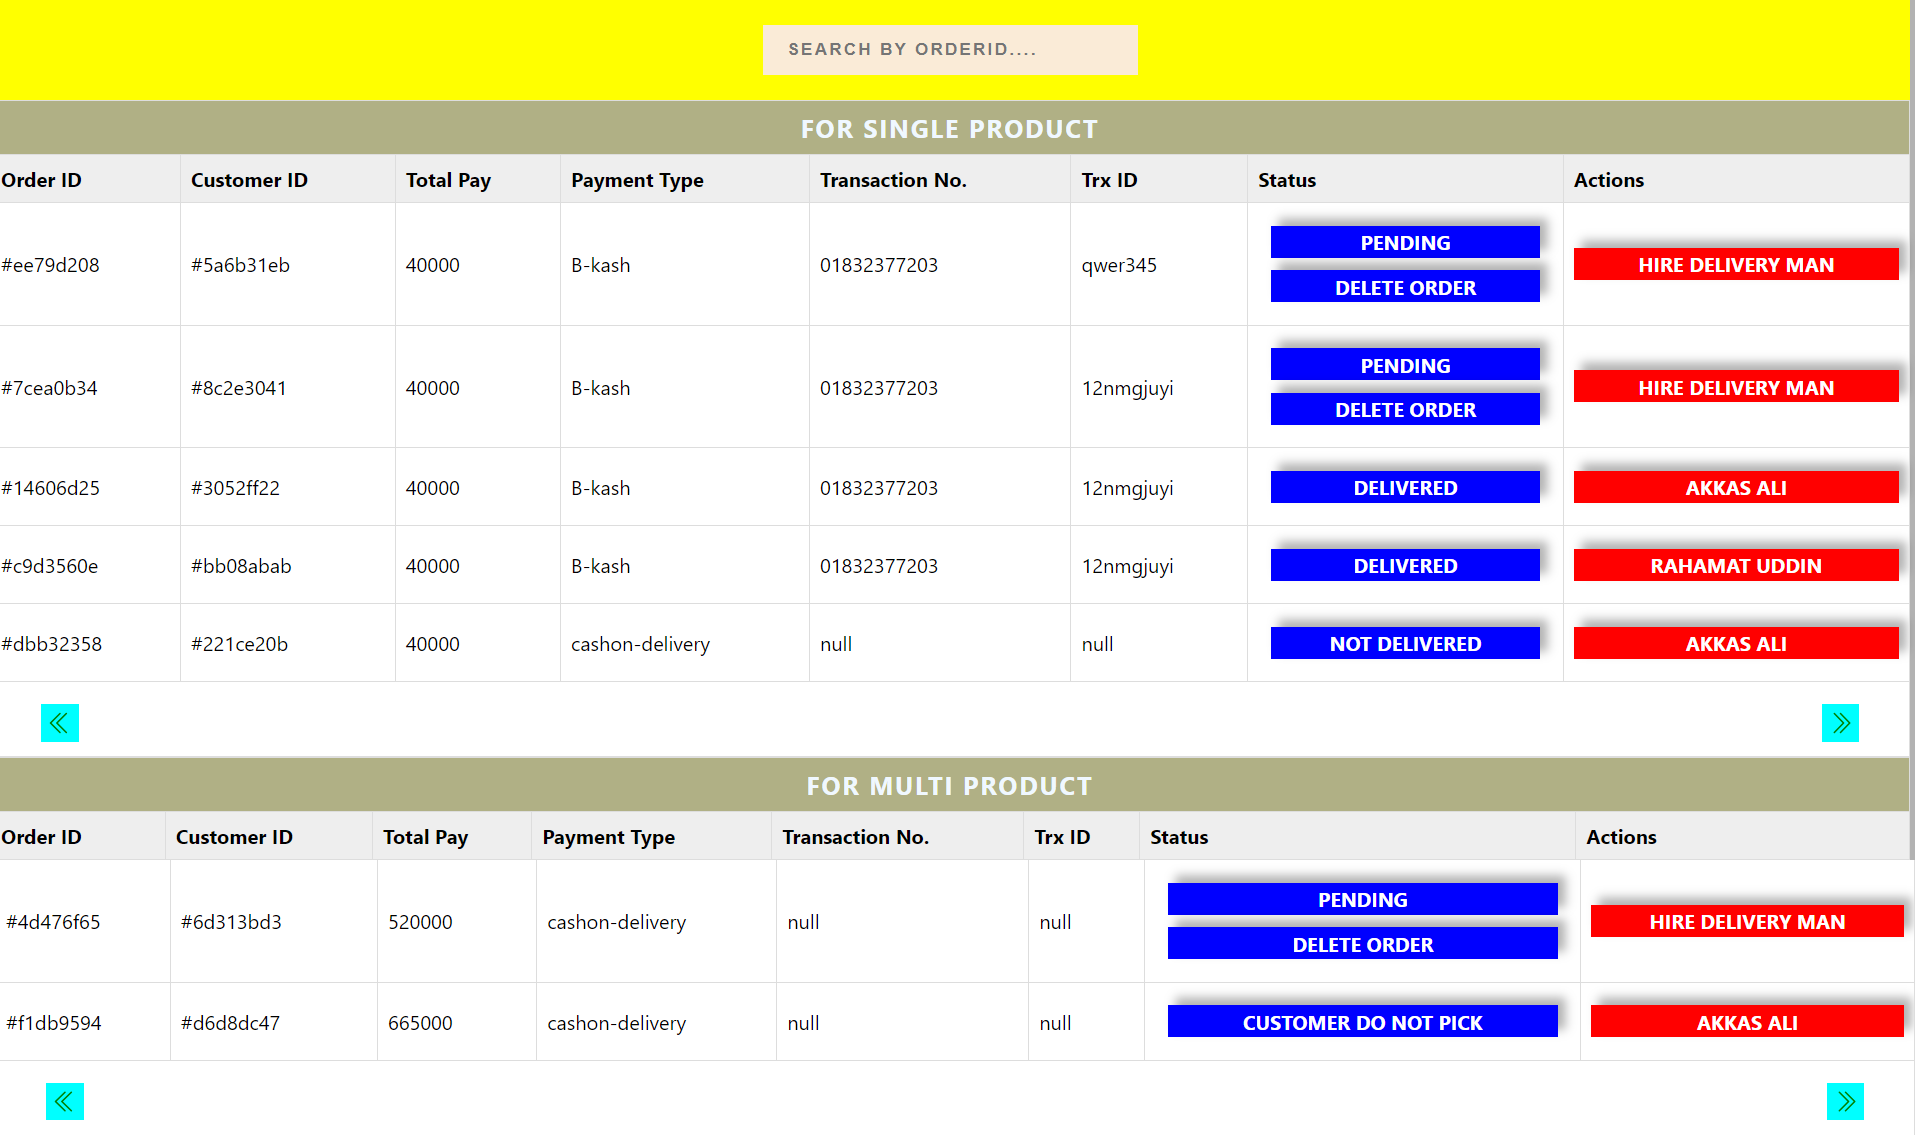
\includegraphics[width=\textwidth, height=0.3\textheight, keepaspectratio]{designs/check -order - staffs.png}    
    \caption{Check orders}
    \label{fig:fig 6.2.20}
\end{figure}

\newpage

\textbf{Hire deliveryman and select service in Shop Management System (Figure \ref{fig:fig 6.2.21})}
\vspace{2cm}
\begin{figure}[ht]
    \centering  
    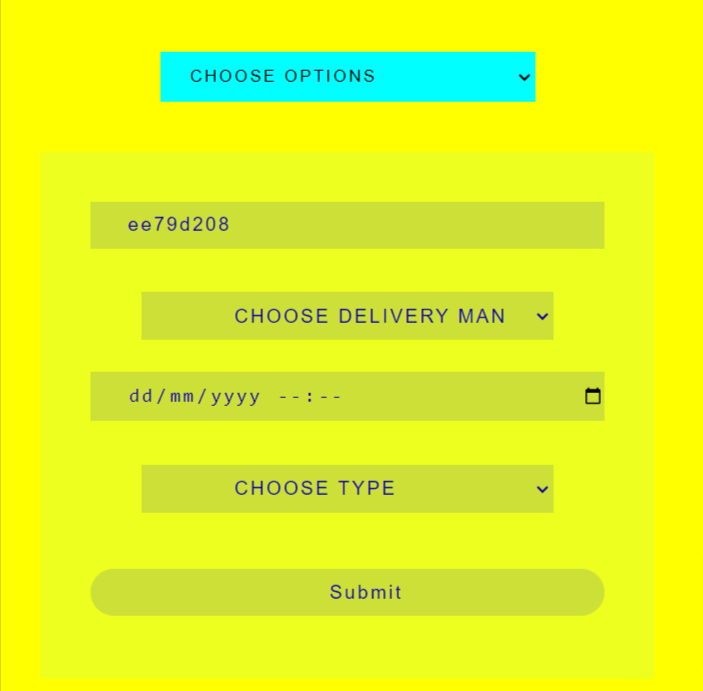
\includegraphics[width=\textwidth, height=0.9\textheight, keepaspectratio]{designs/hire deliveryman and select service for existing order staffs.png}    
    \caption{Hire Delivery man or selects services}
    \label{fig:fig 6.2.21}
\end{figure}

\newpage
\textbf{Handled daily costs in Shop Management System (Figure \ref{fig:fig 6.2.22})}\\

\begin{figure}[ht]
    \centering  
    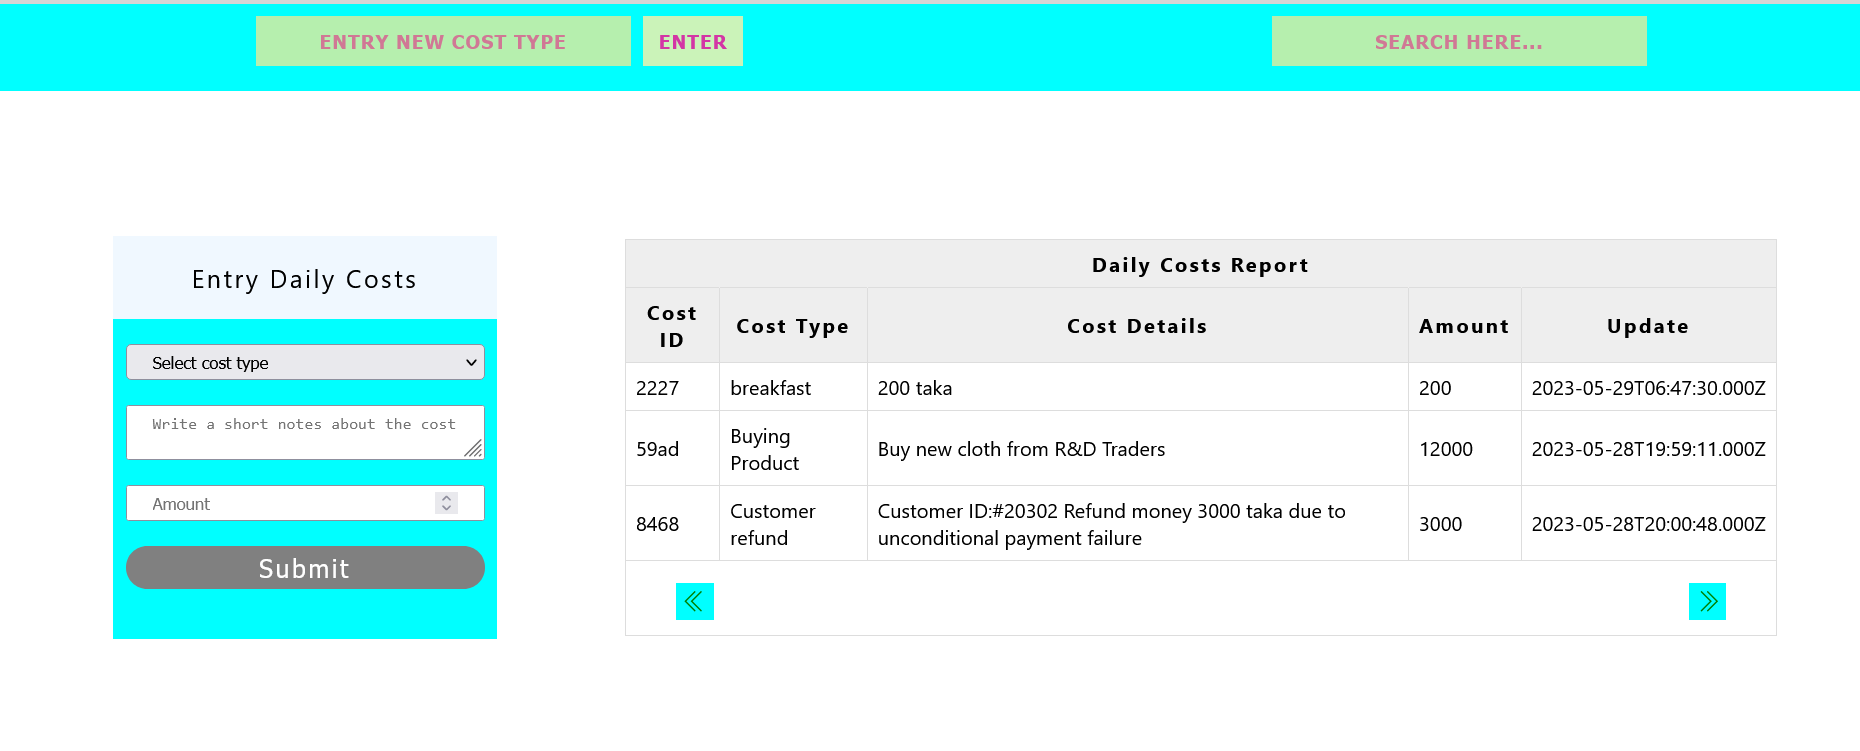
\includegraphics[width=\textwidth, height=0.8\textheight, keepaspectratio]{designs/costs manufacture.png}    
    \caption{Costs specifications}
    \label{fig:fig 6.2.22}
\end{figure}

\textbf{Product CRUD operations in Shop Management System (Figure \ref{fig:fig 6.2.23})}\\

\begin{figure}[ht]
    \centering  
    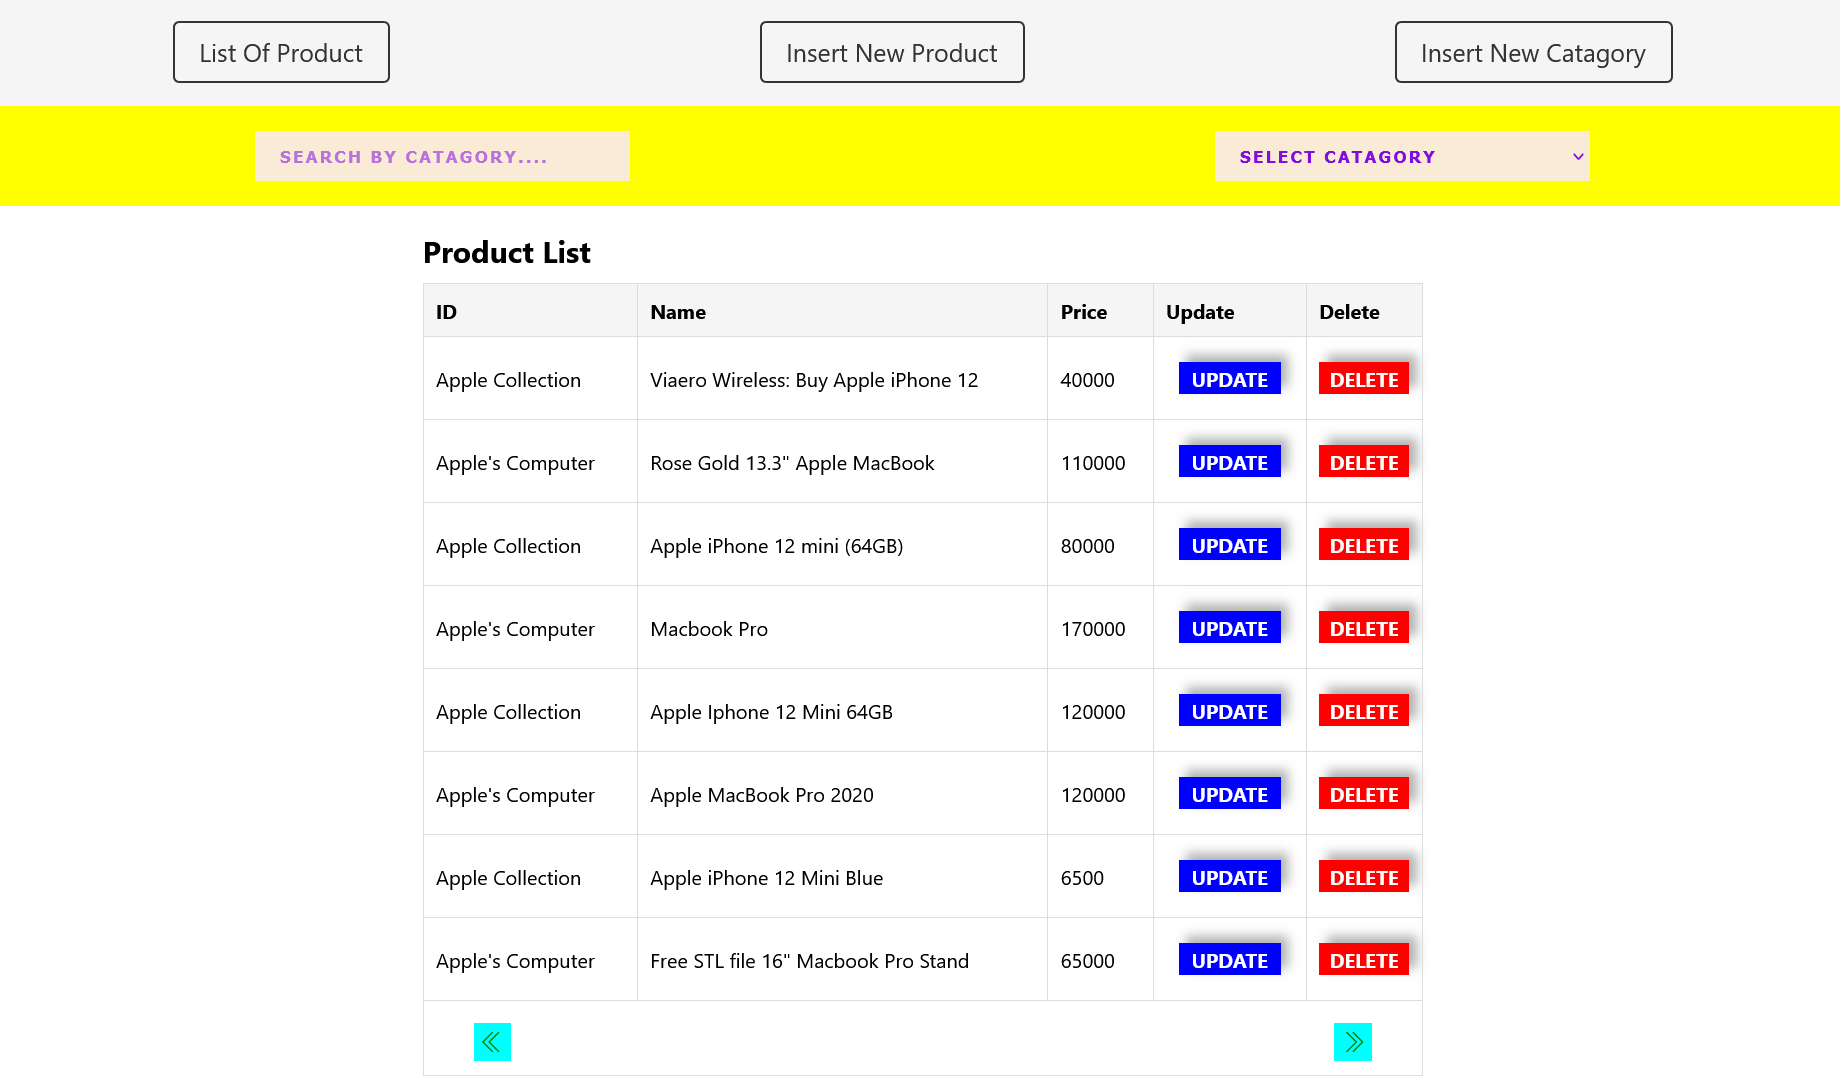
\includegraphics[width=\textwidth, height=0.8\textheight, keepaspectratio]{designs/products crud operation.png}    
    \caption{CRUD operations on Products}
    \label{fig:fig 6.2.23}
\end{figure}

\newpage
\begin{figure}[ht]
\vspace{5cm}
    \centering  
    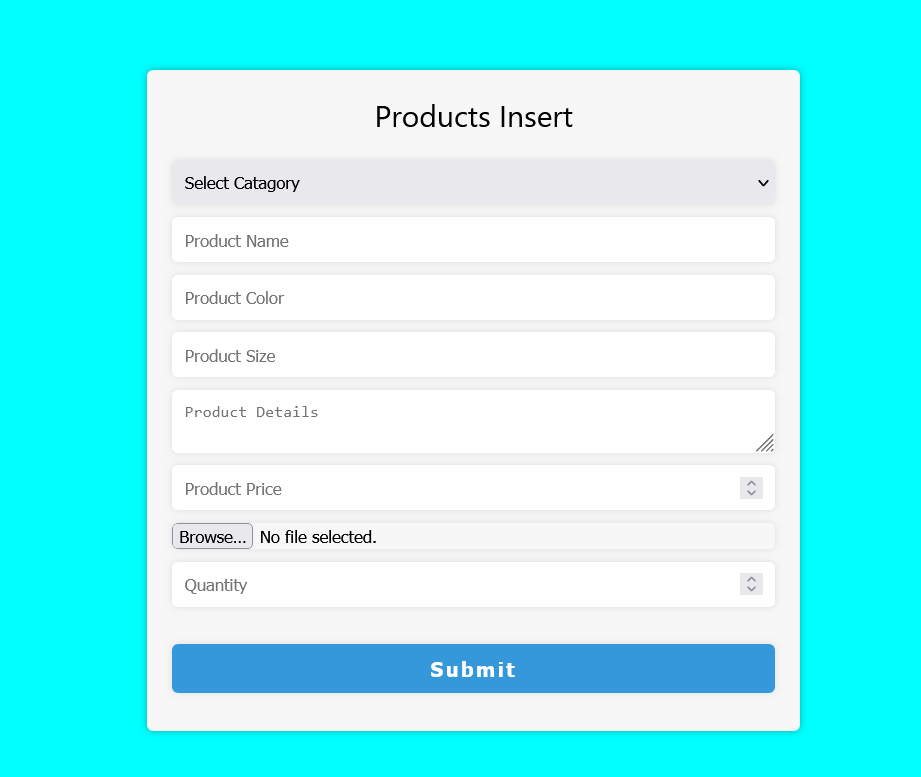
\includegraphics[width=\textwidth, height=0.8\textheight, keepaspectratio]{designs/product insert.png}    
    \caption{Insert New Products}
    \label{fig:fig 6.2.24}
\end{figure}
\begin{figure}[ht]
    \centering  
    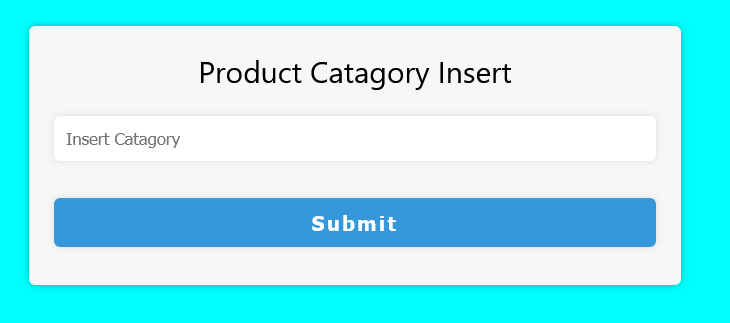
\includegraphics[width=\textwidth, height=0.8\textheight, keepaspectratio]{designs/product catagory insert.png}    
    \caption{Insert New Products Category}
    \label{fig:fig 6.2.25}
\end{figure}
\begin{figure}[ht]
    \centering  
    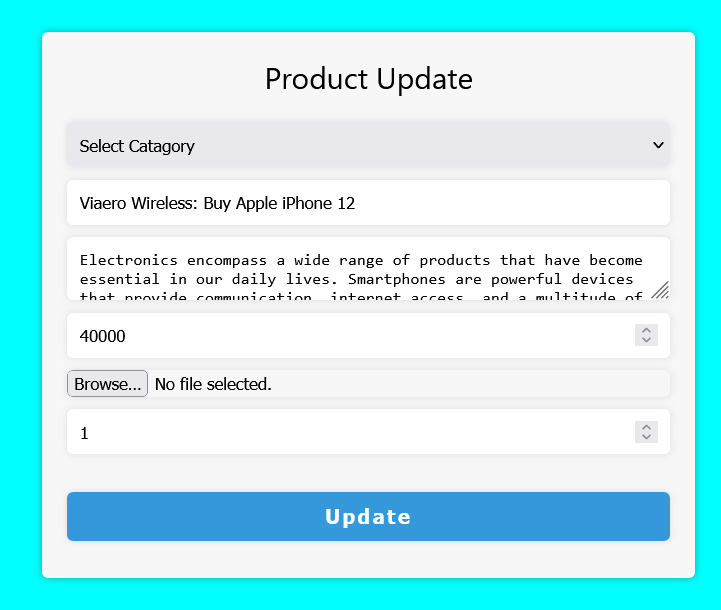
\includegraphics[width=\textwidth, height=0.8\textheight, keepaspectratio]{designs/update produtcs.png}    
    \caption{Update existing product}
    \label{fig:fig 6.2.26}
\end{figure}
\begin{figure}[ht]
    \centering  
    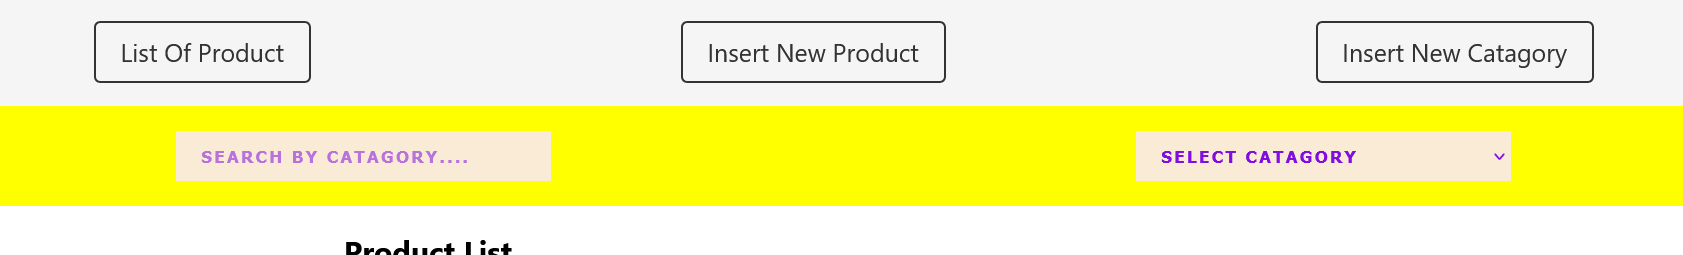
\includegraphics[width=\textwidth, height=0.8\textheight, keepaspectratio]{designs/find products.png}    
    \caption{Find products via search and category wise}
    \label{fig:fig 6.2.27}
\end{figure}
\begin{figure}[ht]
    \centering  
    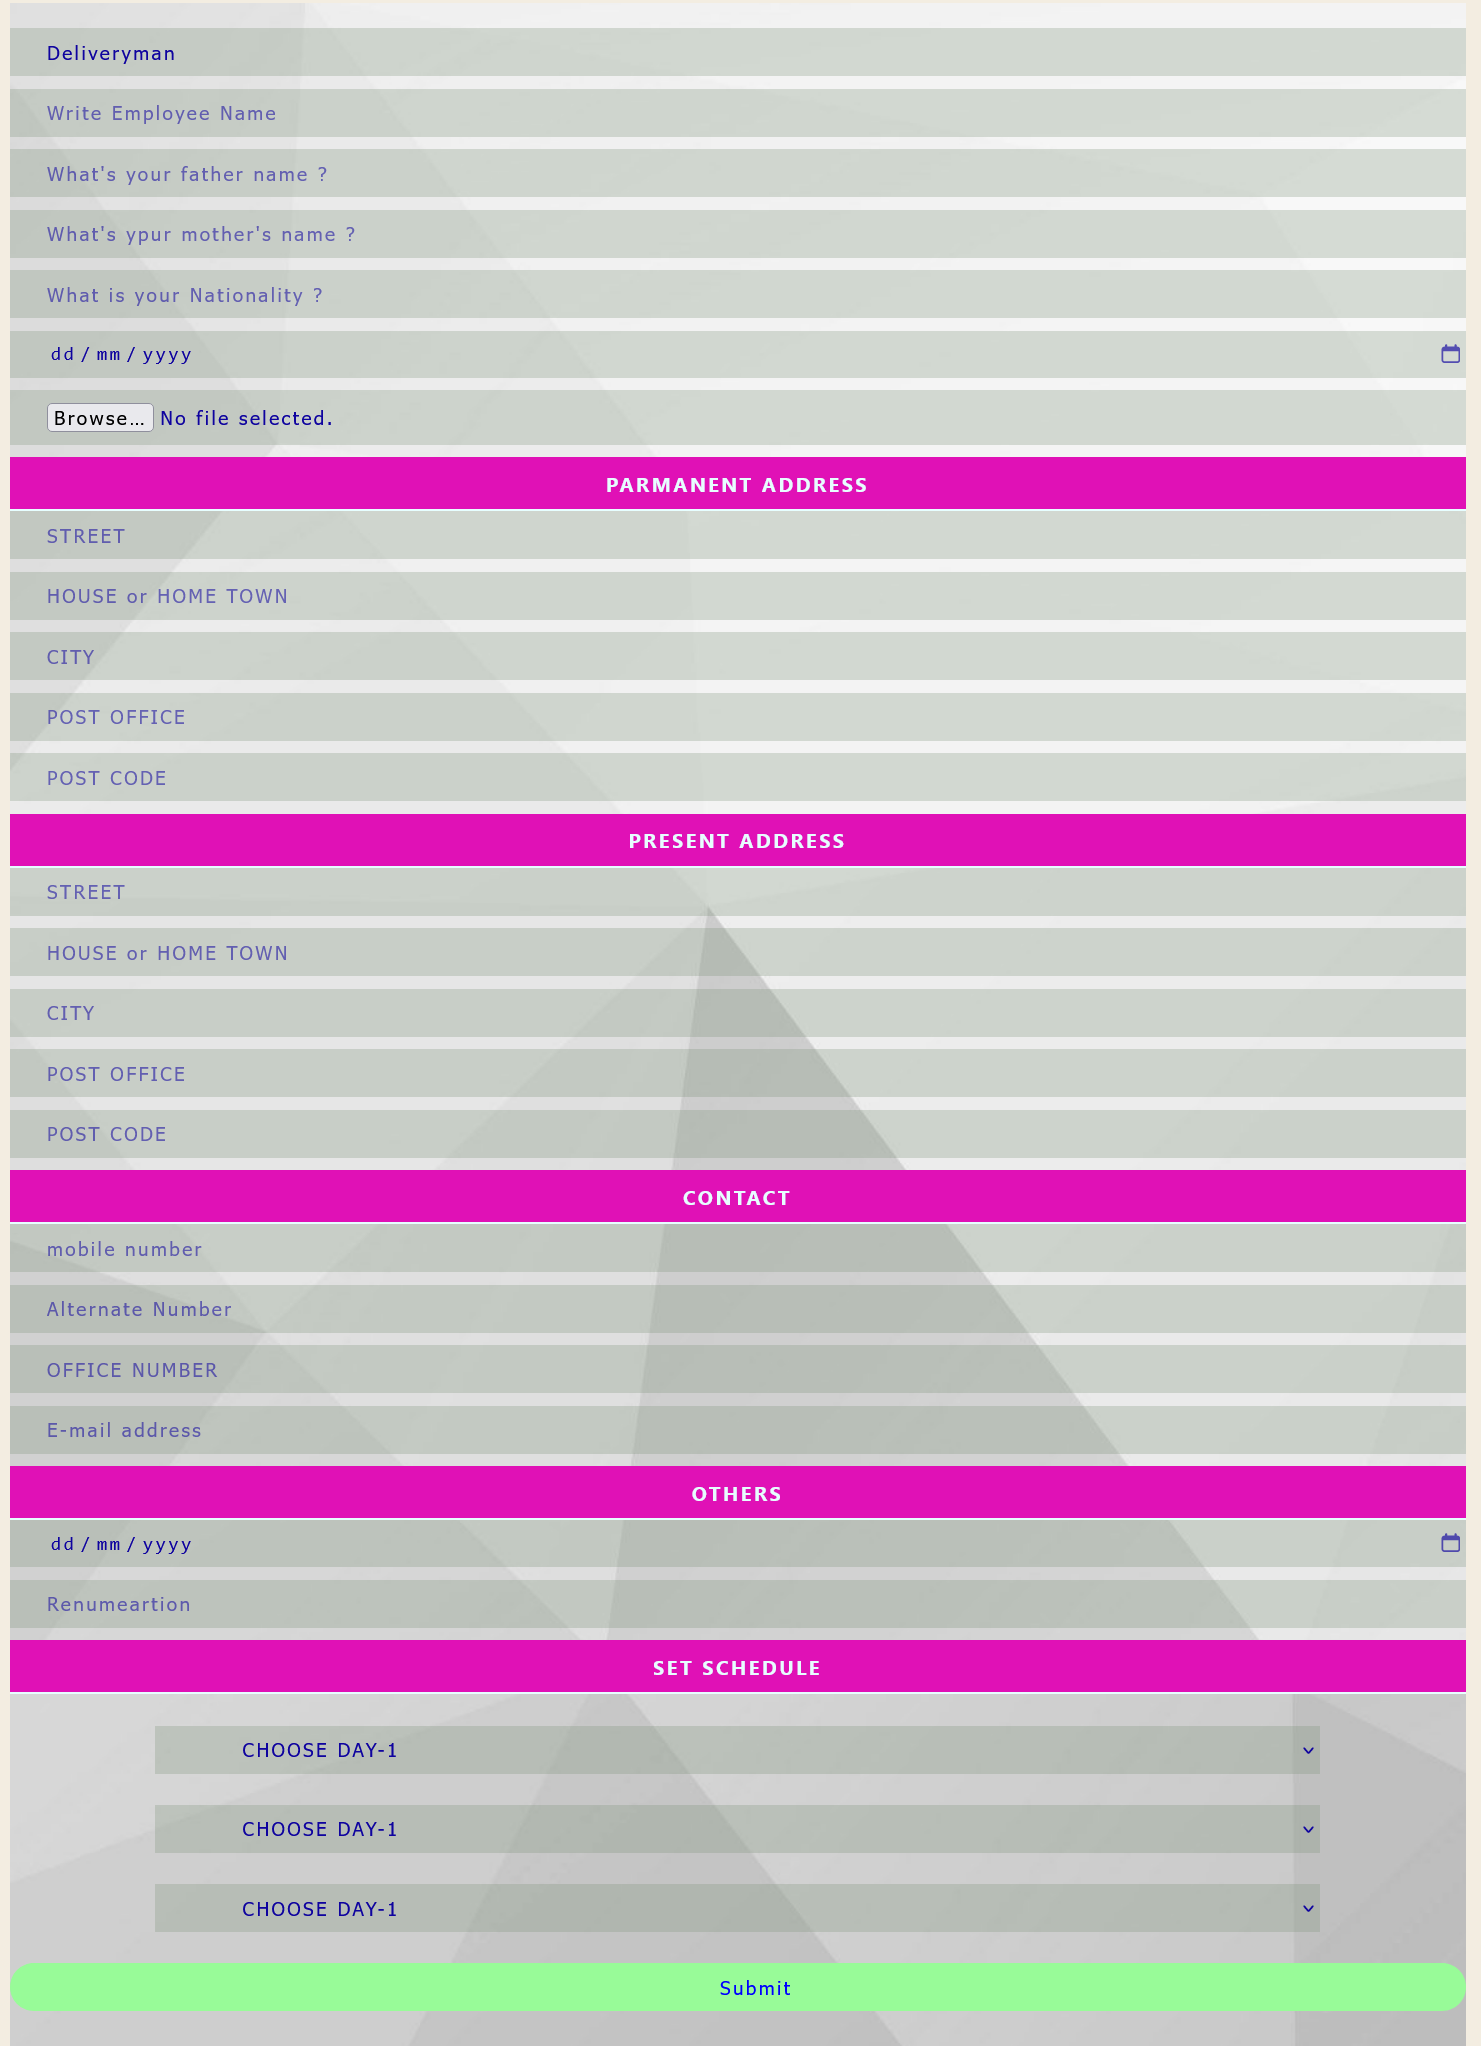
\includegraphics[width=\textwidth, height=0.8\textheight, keepaspectratio]{designs/Add new deliveryman.png}    
    \caption{Hire new deliveryman form}
    \label{fig:fig 6.2.28}
\end{figure}
\begin{figure}[ht]
    \centering  
    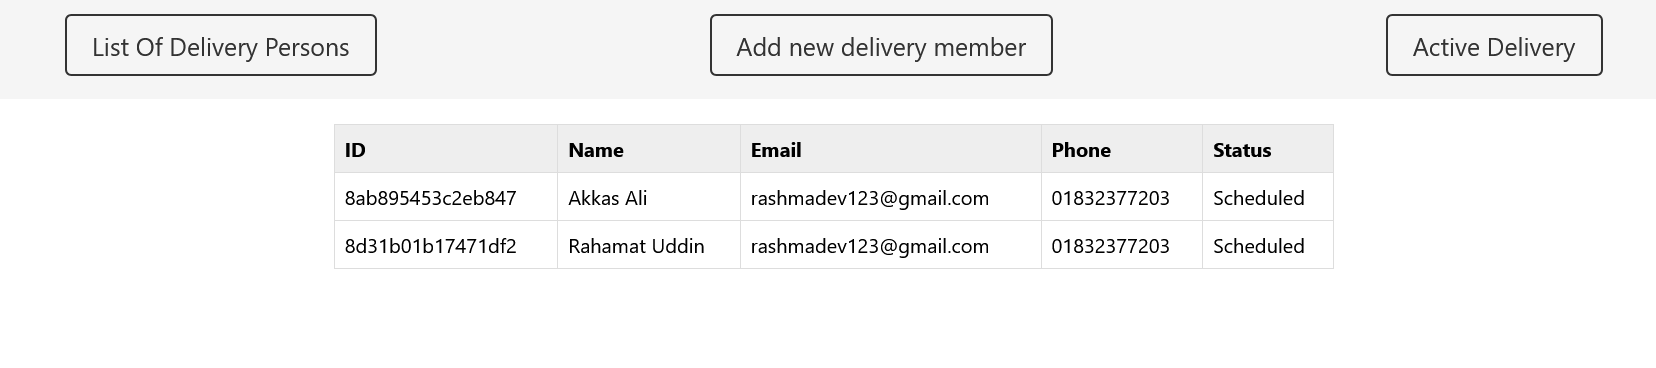
\includegraphics[width=\textwidth, height=0.8\textheight, keepaspectratio]{designs/list of delivery person.png}    
    \caption{Active delivery persons}
    \label{fig:fig 6.2.29}
\end{figure}
\begin{figure}[ht]
    \centering  
    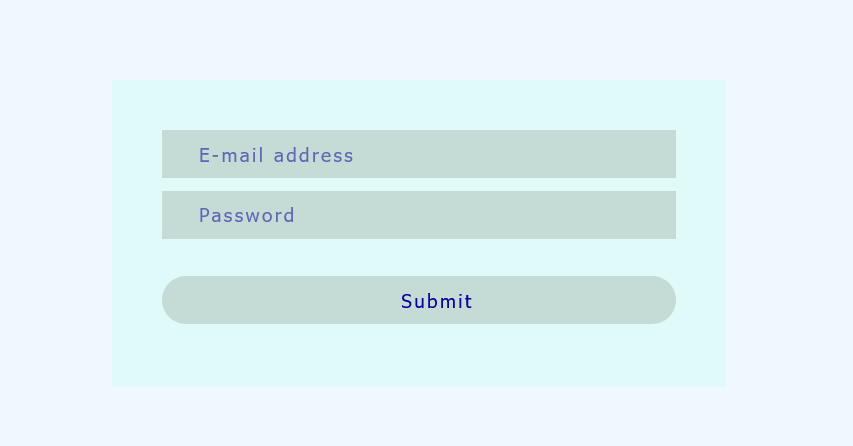
\includegraphics[width=\textwidth, height=0.8\textheight, keepaspectratio]{designs/deliveryman login.png}    
    \caption{Delivery man Login}
    \label{fig:fig 6.2.30}
\end{figure}
\begin{figure}[ht]
    \centering  
    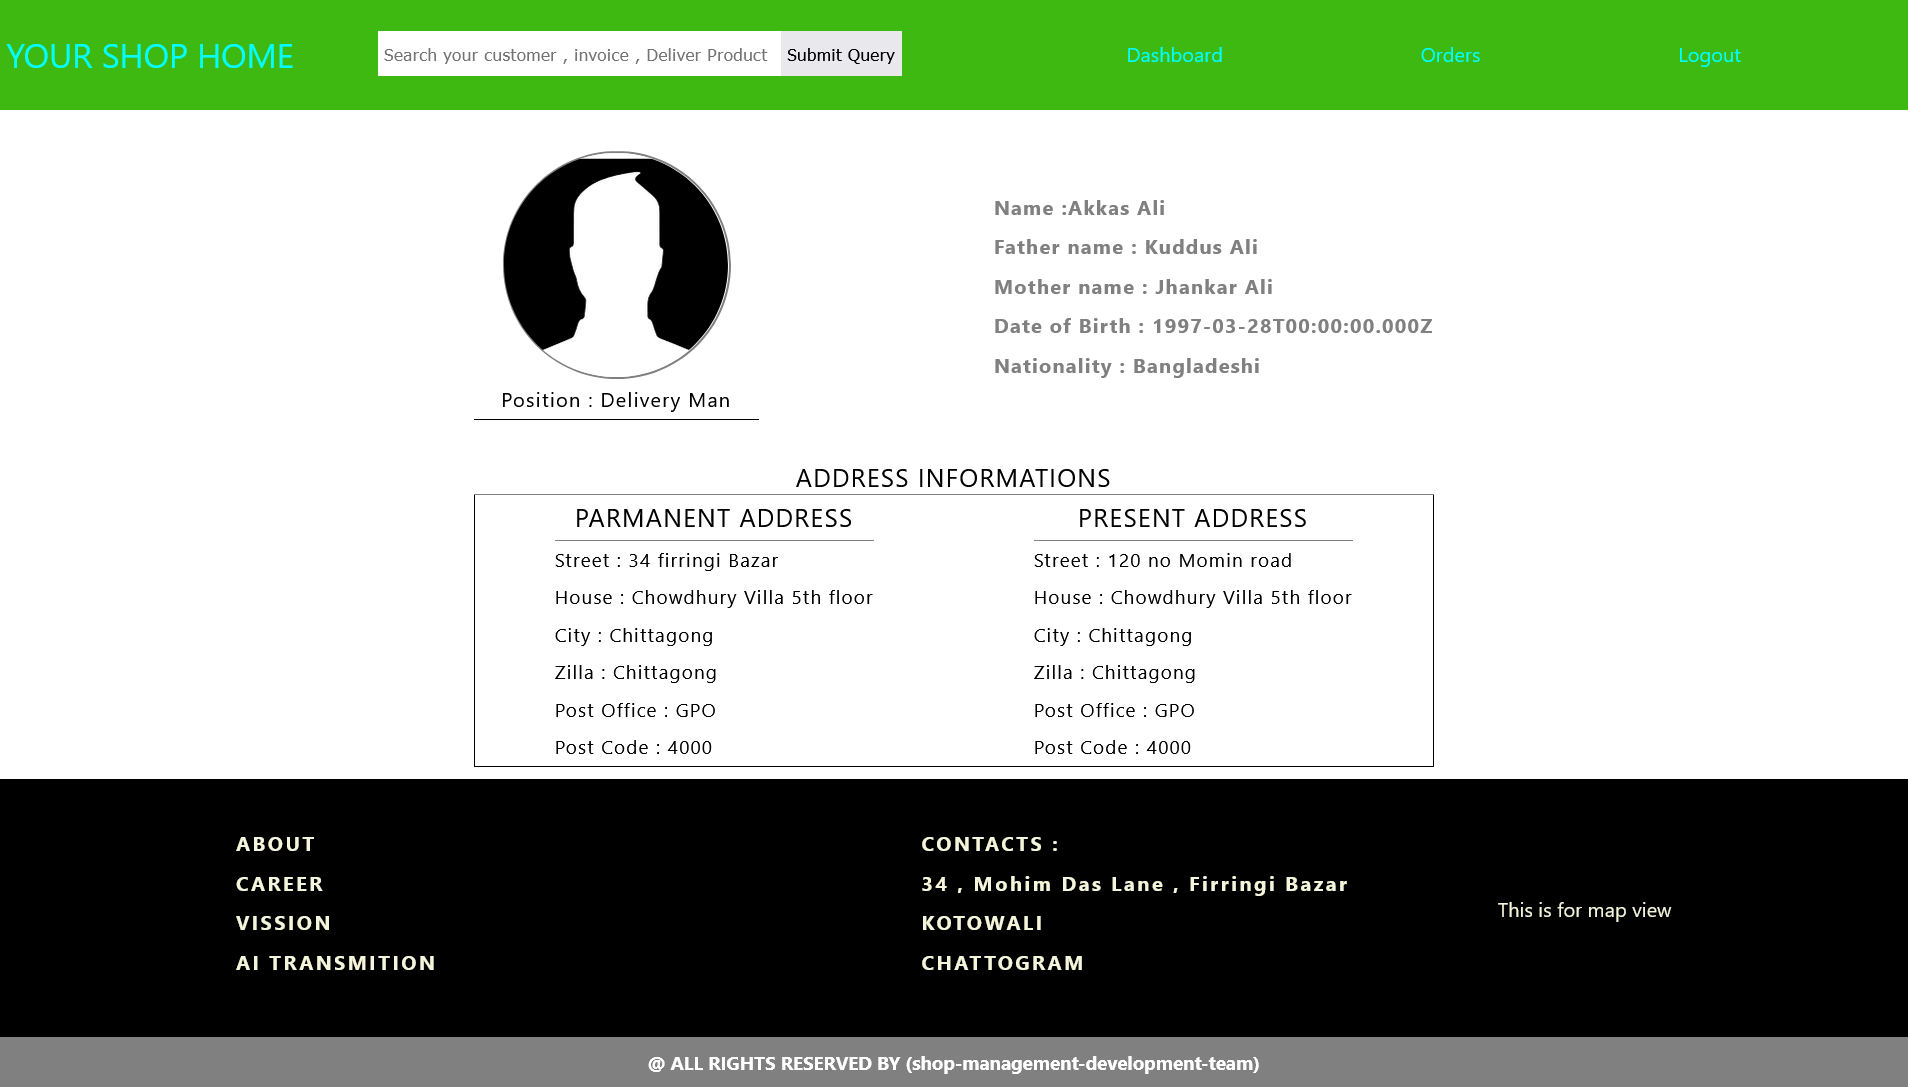
\includegraphics[width=\textwidth, height=0.8\textheight, keepaspectratio]{designs/deliveryman-dashboard.png}    
    \caption{Delivery man Dashboard}
    \label{fig:fig 6.2.31}
\end{figure}
\begin{figure}[ht]
        \centering  
        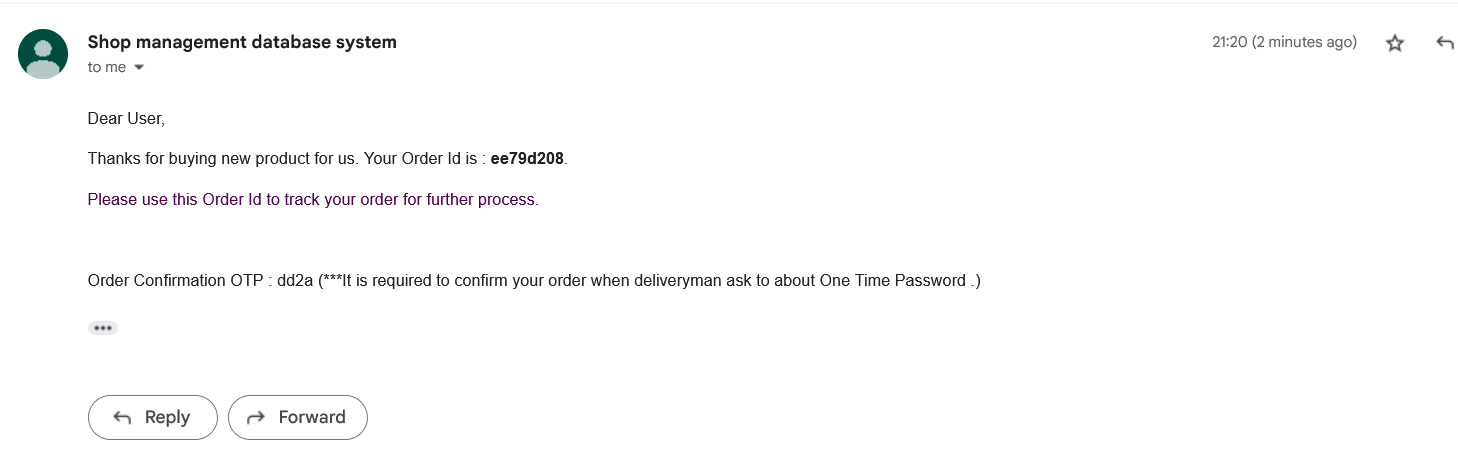
\includegraphics[width=\textwidth]{designs/order confirmation mail.png}    
        \caption{Get order confirmation mail}
        \label{fig:fig 6.2.10}
    \end{figure} 
\begin{figure}[ht]
    \centering  
    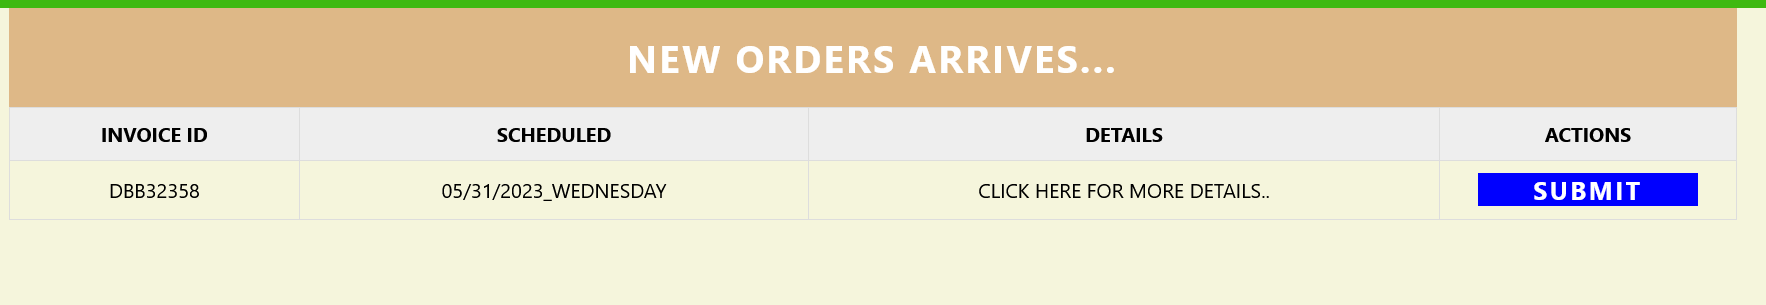
\includegraphics[width=\textwidth, height=0.8\textheight, keepaspectratio]{designs/check new orders.png}    
    \caption{Check new orders}
    \label{fig:fig 6.2.32}
\end{figure}
\begin{figure}[ht]
    \centering  
    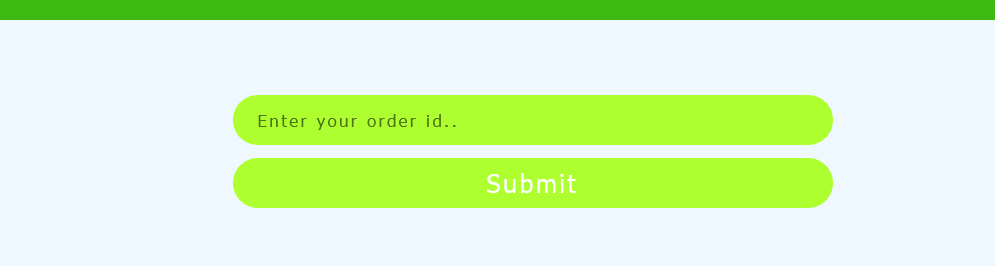
\includegraphics[width=\textwidth, height=0.8\textheight, keepaspectratio]{designs/customer gets OTP.png}    
    \caption{Enter the order id To Validate customers}
    \label{fig:fig 6.2.33}
\end{figure}
\begin{figure}[ht]
    \centering  
    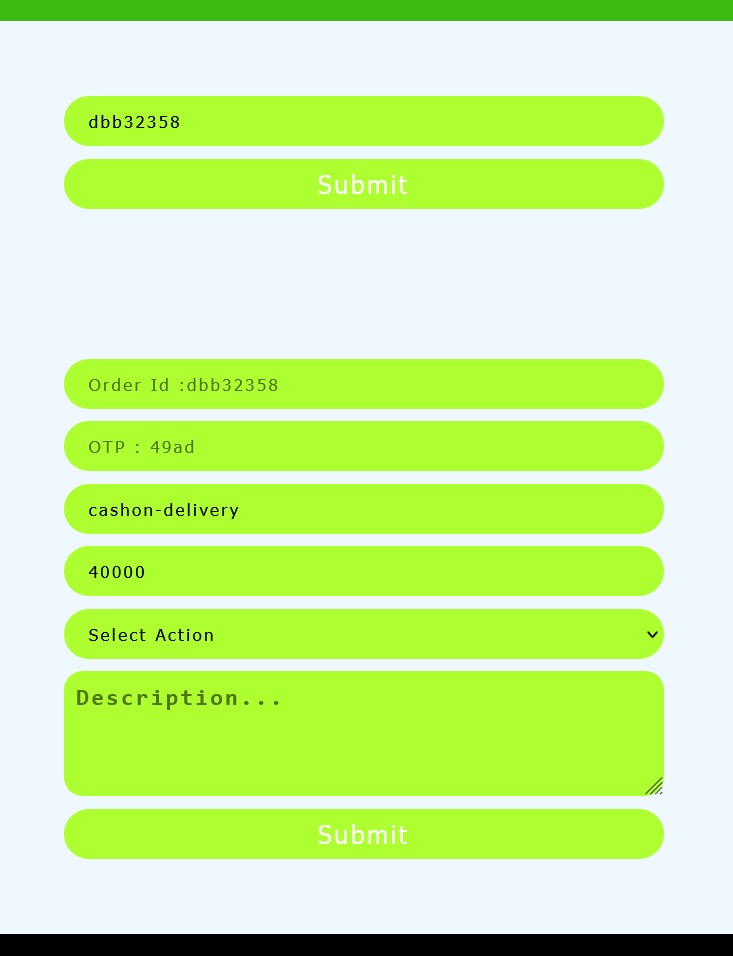
\includegraphics[width=\textwidth, height=0.8\textheight, keepaspectratio]{designs/orders completations.png}    
    \caption{Handled orders to the customers}
    \label{fig:fig 6.2.34}
\end{figure}
